% ============================================================
%  srn-captions.tex
%  Figure captions for the Sango Rine Shumba (SRN) paper.
%  Include in the main document with % ============================================================
%  srn-captions.tex
%  Figure captions for the Sango Rine Shumba (SRN) paper.
%  Include in the main document with % ============================================================
%  srn-captions.tex
%  Figure captions for the Sango Rine Shumba (SRN) paper.
%  Include in the main document with % ============================================================
%  srn-captions.tex
%  Figure captions for the Sango Rine Shumba (SRN) paper.
%  Include in the main document with \input{srn-captions}.
% ============================================================

% ── Panel 1: Partition Space Geometry ────────────────────────────────────────

\begin{figure*}[!htbp]
    \centering
    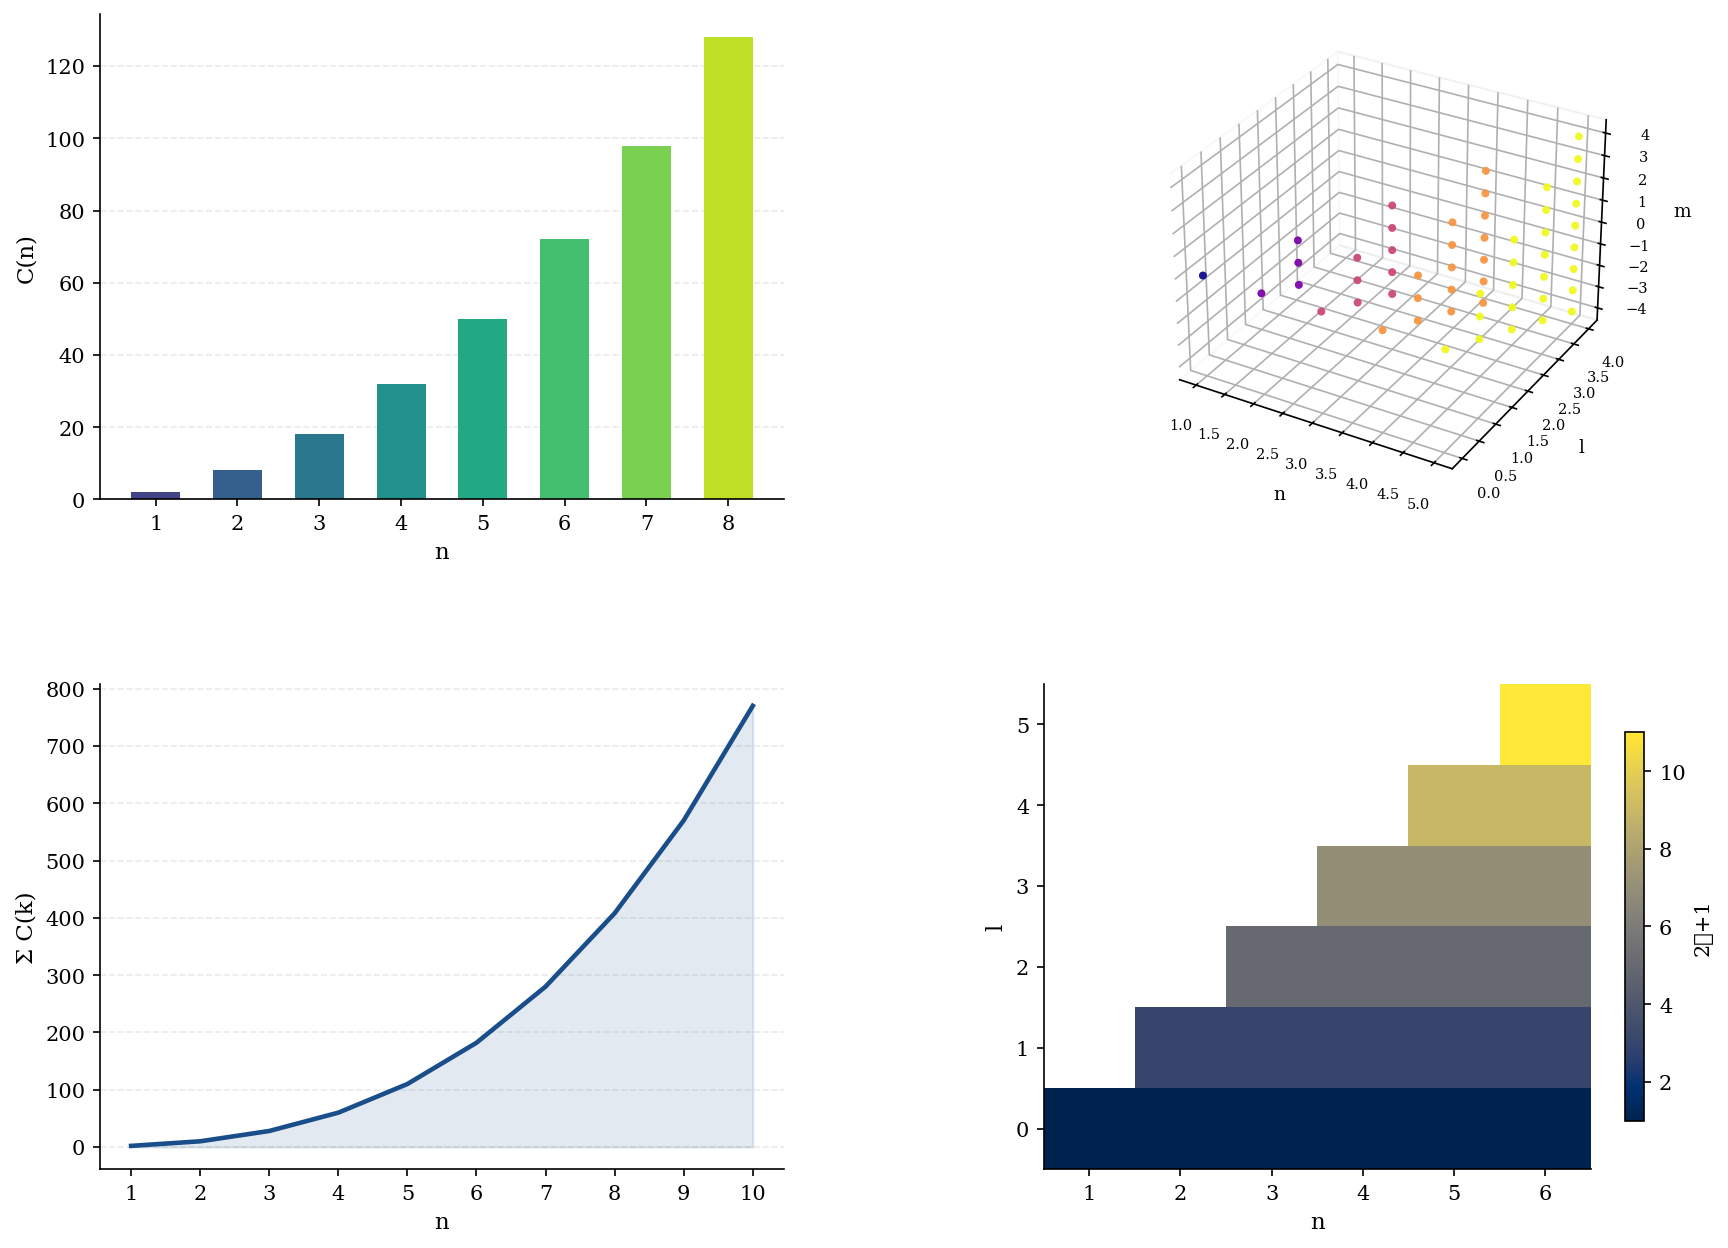
\includegraphics[width=\textwidth]{panel1_partition_geometry.png}
    \caption{\textbf{Partition Space Geometry.}
    (\textbf{A})~Shell capacity $C(n) = 2n^2$ for partition depths
    $n = 1, \ldots, 8$.  Each bar counts the number of valid coordinate
    quadruples $(\ell, m, s)$ at depth $n$: $\ell$ ranges over
    $\{0, \ldots, n-1\}$, $m$ over $\{-\ell, \ldots, +\ell\}$, and
    $s \in \{-\tfrac{1}{2}, +\tfrac{1}{2}\}$, giving
    $2\sum_{\ell=0}^{n-1}(2\ell+1) = 2n^2$ distinct addresses per shell.
    Bars are coloured from cool (shallow) to warm (deep) to indicate
    structural richness increasing with depth.
    (\textbf{B})~Three-dimensional scatter of all valid partition
    coordinates $(n, \ell, m)$ for $n \leq 5$, with spin parity $s$
    doubling each point's multiplicity.  Each point represents a unique
    node identity in the \srn\ network.  Depth $n$ determines the
    colour; the triangular cross-section at each depth reflects the
    constraint $|\,m\,| \leq \ell < n$.  The geometry is the discrete
    analogue of the hydrogen-atom orbital manifold arising from
    $\mathrm{SO}(3)$ representation theory.
    (\textbf{C})~Cumulative coordinate count
    $\sum_{k=1}^{n} 2k^2 = \tfrac{n(n+1)(2n+1)}{3}$ as a function of
    depth $n$.  By $n = 4$, the address space has $110$ distinct nodes;
    by $n = 6$, it reaches $182$.  The filled area emphasises the
    super-linear growth of the address space with depth.
    (\textbf{D})~Heatmap of the number of valid orientation indices
    $2\ell + 1$ over the $(n, \ell)$ grid for $n, \ell \in \{1,\ldots,6\}$.
    Grey (NaN) cells are structurally forbidden ($\ell \geq n$): they
    cannot be individuated at the given depth.  Permitted cells grow
    darker as $\ell$ increases, reflecting the widening orientation fan.
    The triangular forbidden region is the discrete shadow of the angular
    momentum constraint $\ell \in \{0, \ldots, n-1\}$.}
    \label{fig:panel1}
\end{figure*}

% ── Panel 2: Entropic Floor and Catalytic Dynamics ───────────────────────────

\begin{figure*}[!htbp]
    \centering
    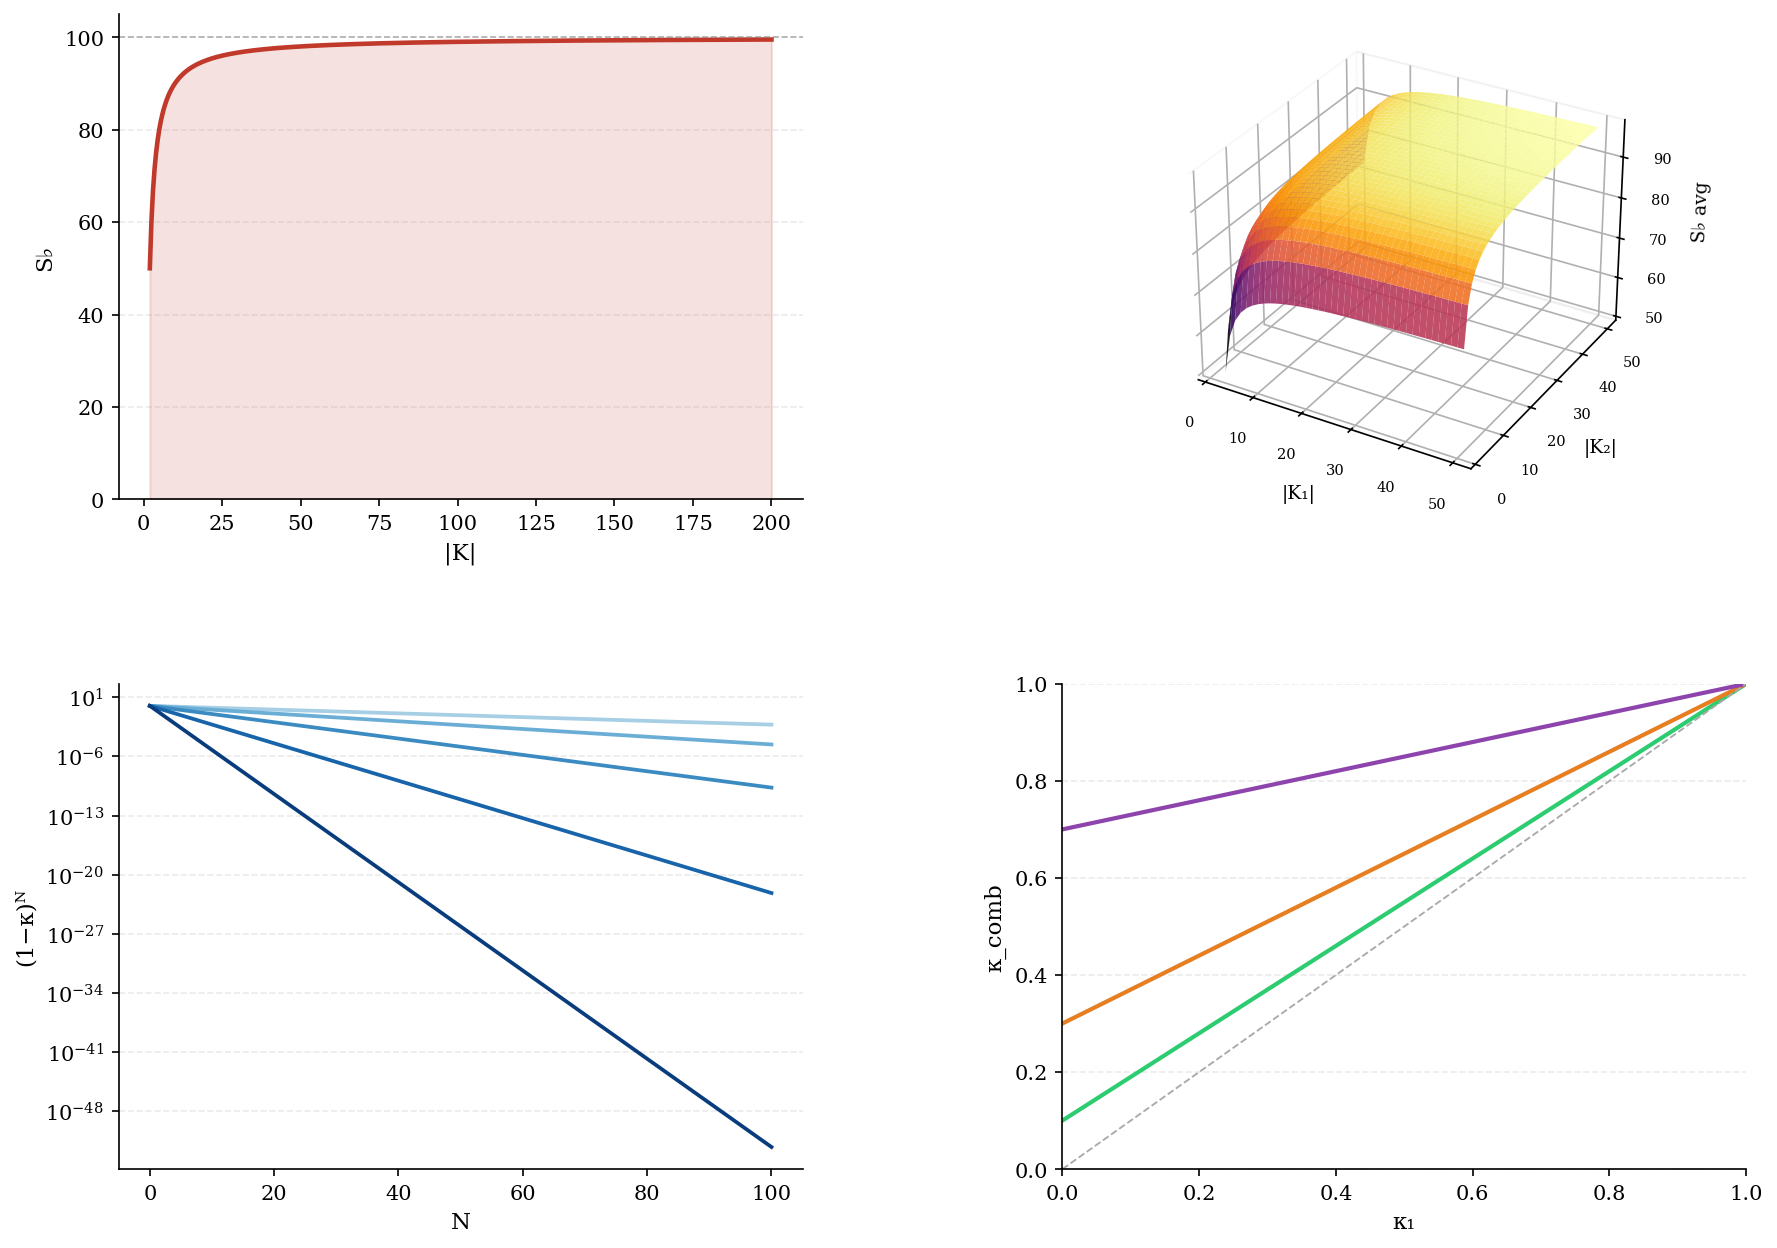
\includegraphics[width=\textwidth]{panel2_entropic_floor.png}
    \caption{\textbf{Entropic Floor and Catalytic Dynamics.}
    (\textbf{A})~The entropic floor $\floor(K) = 100(1 - 1/|K|)$ as a
    function of the receiver's knowledge framework size $|K|$, for
    $|K| \in [2, 200]$.  The filled region marks the range of
    achievable S-values.  The dashed line at $\floor = 100$ is the
    unattainable limit: perfect knowledge requires $|K| = \infty$.  At
    $|K| = 2$, the floor is $50$; at $|K| = 10$, it is $90$; at
    $|K| = 100$, it is $99$.  No finite receiver can close the gap to
    zero error, regardless of expression quality.
    (\textbf{B})~Three-dimensional surface of the average floor
    $\tfrac{1}{2}({\floor}(K_1) + {\floor}(K_2)) =
    50(2 - 1/|K_1| - 1/|K_2|)$ over two independent receiver sizes
    $|K_1|, |K_2| \in [2, 50]$.  The surface rises monotonically in both
    directions and remains strictly below $100$ everywhere.  The two
    receivers each contribute an independent positive floor; the average
    is the relevant quantity for cross-node evaluation, where neither
    receiver can achieve zero error in isolation.
    (\textbf{C})~Log-scale catalytic residual $(1-\kappa)^N$ as a
    function of step count $N \in [0, 100]$ for five catalyst strengths
    $\kappa \in \{0.05, 0.1, 0.2, 0.4, 0.7\}$ (light to dark).  All
    curves converge to zero, confirming the Borel-Cantelli analogue
    (Theorem~\ref{thm:catalyst}): repeated application of any catalyst
    with $\kappa > 0$ drives the residual to zero exponentially fast.
    The rate is $(1-\kappa)$ per step: a catalyst of strength $0.7$
    reduces the residual to $< 10^{-5}$ within $30$ steps; one of
    strength $0.05$ requires $\sim 200$ steps for the same reduction.
    (\textbf{D})~Composite catalytic power
    $\kappa_{\mathrm{comb}}(\kappa_1, \kappa_2)
    = 1 - (1 - \kappa_1)(1 - \kappa_2)$ as $\kappa_1$ varies over
    $[0,1]$ for three fixed values $\kappa_2 \in \{0.1, 0.3, 0.7\}$
    (green, orange, purple).  The diagonal reference line marks
    $\kappa_{\mathrm{comb}} = \kappa_1$.  Every curve lies strictly
    above the diagonal for $\kappa_1 \in (0,1)$, confirming that
    combining two catalysts always outperforms either alone.  A locally
    infeasible catalyst ($\kappa_2$ from a node where $S = 100$) retains
    positive composite power by the Miracle Principle
    (Corollary~\ref{cor:miracle}).}
    \label{fig:panel2}
\end{figure*}

% ── Panel 3: Composition Inflation ───────────────────────────────────────────

\begin{figure*}[!htbp]
    \centering
    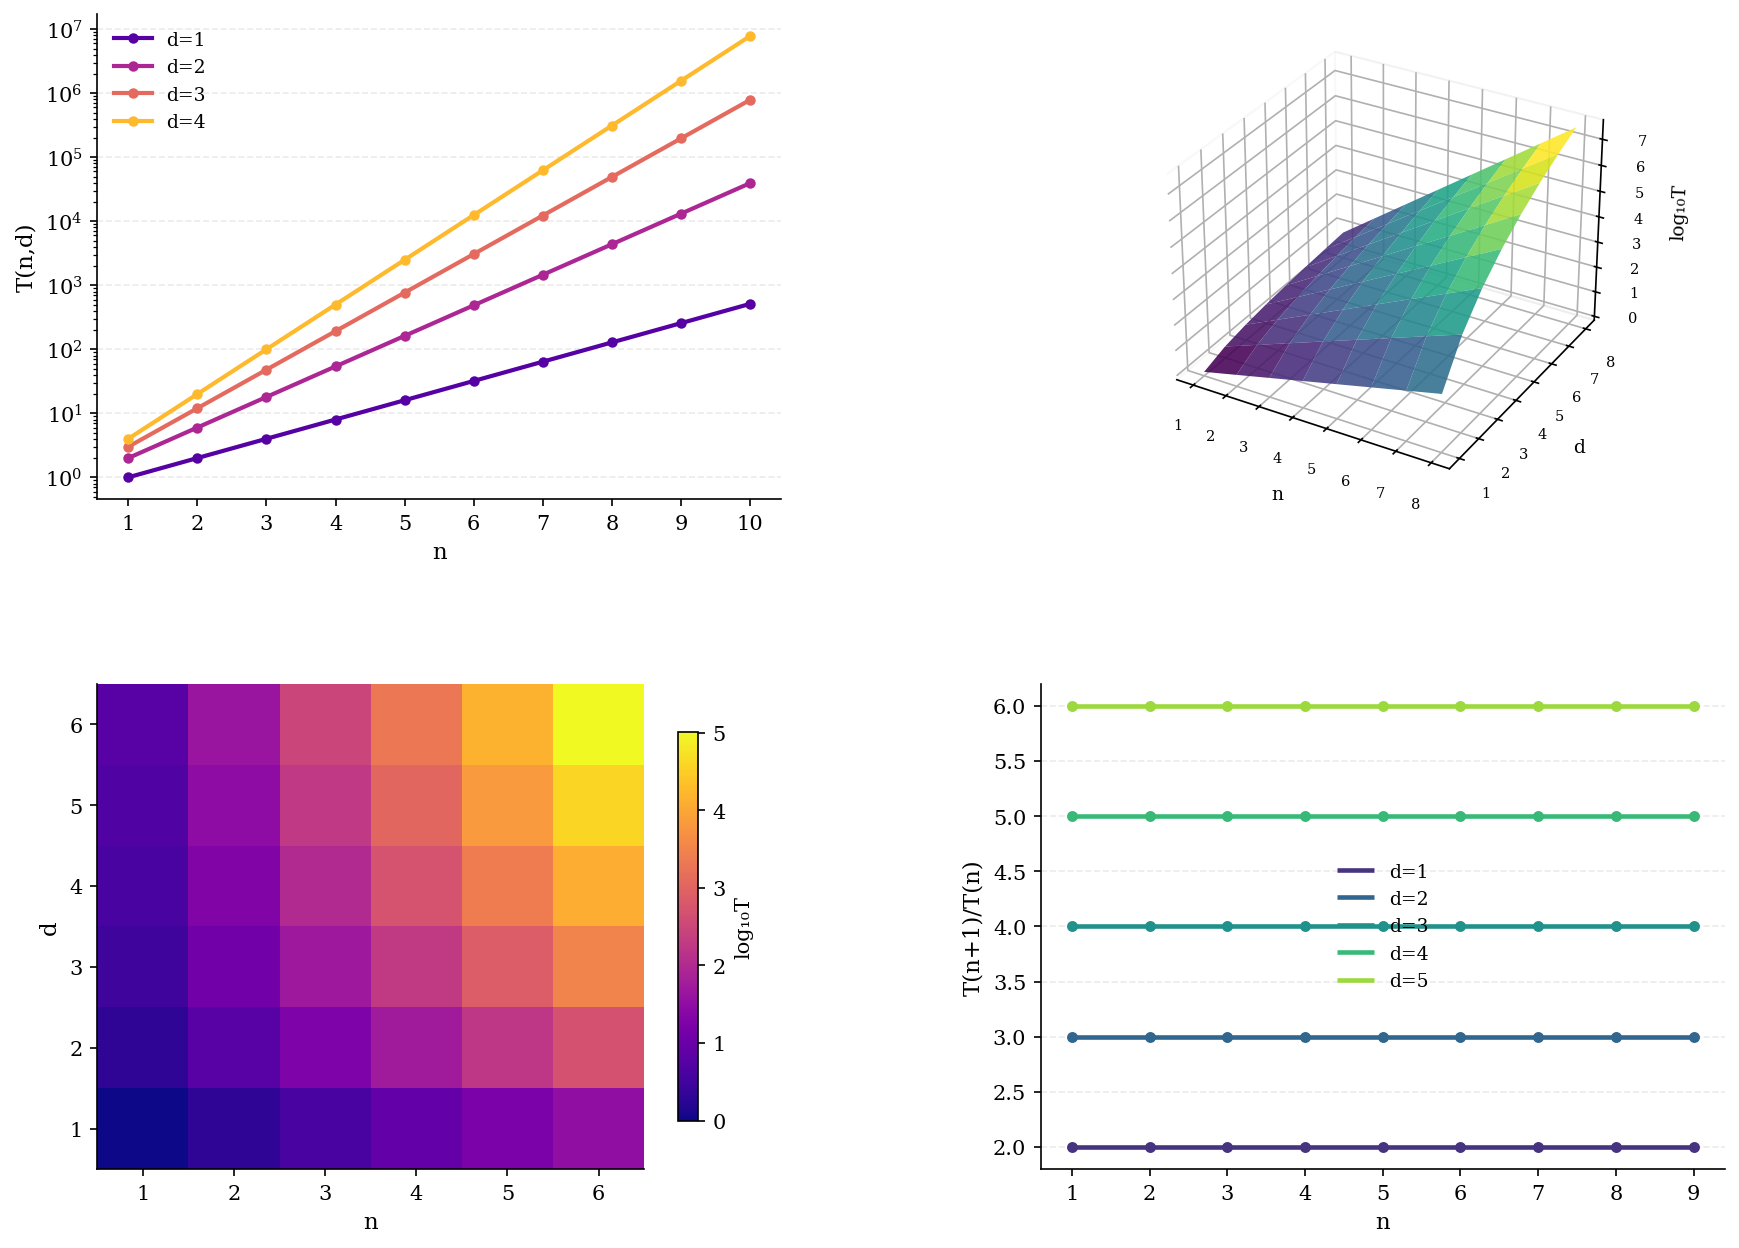
\includegraphics[width=\textwidth]{panel3_composition_inflation.png}
    \caption{\textbf{Composition Inflation $T(n,d) = d(1+d)^{n-1}$.}
    (\textbf{A})~Log-scale growth of $T(n,d)$ versus composition depth
    $n \in \{1, \ldots, 10\}$ for operator counts $d \in \{1, 2, 3, 4\}$.
    All curves are strictly exponential in $n$; the base $(1+d)$
    increases with $d$, so higher operator counts produce faster
    trajectory proliferation.  At $n = 10$ and $d = 4$, the number of
    distinguishable labeled trajectories exceeds $2 \times 10^6$.  The
    linear regime ($n = 1$, where $T = d$ regardless of base) is the
    unique fixed point visible at the left edge.
    (\textbf{B})~Three-dimensional surface of $\log_{10} T(n,d)$ over
    $(n, d) \in \{1, \ldots, 8\}^2$.  The surface is coloured by height:
    cool shades indicate few trajectories; warm shades indicate many.
    The exponential dependence on $n$ and the linear-then-exponential
    dependence on $d$ produce a surface that rises steeply in both
    directions, but more steeply along $n$ for fixed $d > 1$.
    (\textbf{C})~Heatmap of $\log_{10} T(n,d)$ for
    $(n, d) \in \{1,\ldots,6\}^2$.  Each cell is coloured by the
    base-10 logarithm of the trajectory count.  The heatmap reveals
    the multiplicative structure: moving one step right (increasing $n$
    by $1$) multiplies $T$ by $(1+d)$; moving one step up (increasing
    $d$ by $1$) adds an additional factor that varies with $n$.  The
    fastest-growing cell at $(n=6, d=6)$ has $T = 6 \cdot 7^5 \approx
    7 \times 10^4$ trajectories.
    (\textbf{D})~Growth ratio $T(n+1, d) / T(n, d) = 1 + d$ as a
    function of $n$ for $d \in \{1, 2, 3, 4, 5\}$.  Each curve is a
    horizontal line, confirming that the ratio is exactly constant in
    $n$: the exponential base $(1+d)$ is independent of depth.  This
    is a structural consequence of the binomial identity underlying the
    Composition Inflation theorem (Theorem~\ref{thm:inflation}), not
    a numerical accident.  Dots mark the integer values of $n$ where
    the ratio was evaluated.}
    \label{fig:panel3}
\end{figure*}

% ── Panel 4: Forest Dynamics and Receiver-Relative Evaluation ────────────────

\begin{figure*}[!htbp]
    \centering
    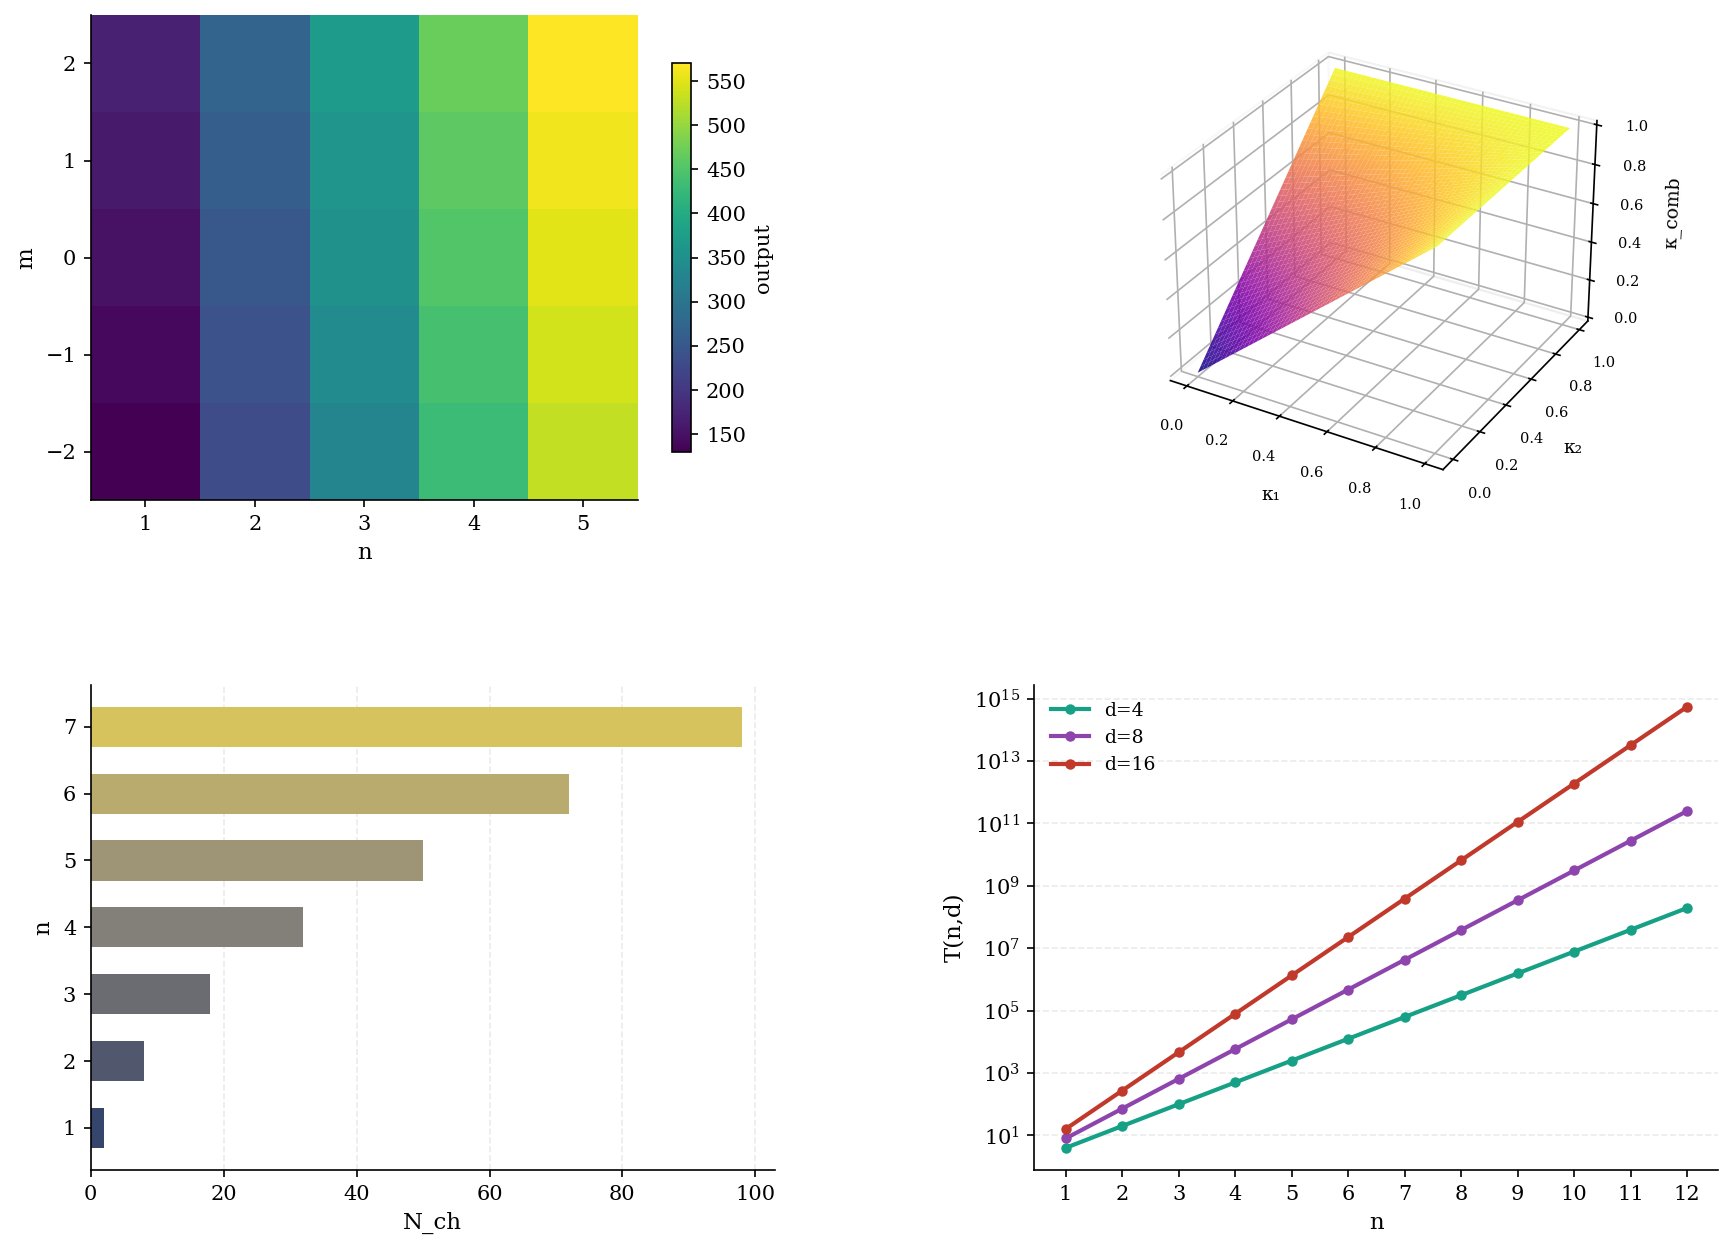
\includegraphics[width=\textwidth]{panel4_forest_dynamics.png}
    \caption{\textbf{Forest Dynamics and Receiver-Relative Evaluation.}
    (\textbf{A})~Heatmap of the receiver-relative output
    $v = 100n + 10m + M$ (with partition count $M = 50$ fixed)
    across the $(n, m)$ node grid, $n \in \{1,\ldots,5\}$,
    $m \in \{-2,-1,0,+1,+2\}$.  Every cell yields a distinct value:
    no two nodes evaluate the same expression to the same result.
    This is a direct numerical illustration of
    Theorem~\ref{thm:rr} (Receiver-Relativity): the same \srn\
    expression produces different output at every node in the network,
    with all outputs simultaneously valid.  The colour gradient
    encodes the output value; no central authority reconciles the
    divergent results.
    (\textbf{B})~Three-dimensional surface of composite catalytic power
    $\kappa_{\mathrm{comb}}(\kappa_1, \kappa_2)
    = 1 - (1 - \kappa_1)(1 - \kappa_2)$ over $(\kappa_1, \kappa_2)
    \in [0,1]^2$.  The surface is bounded in $[0,1]^2$, rises
    monotonically in both arguments, and reaches $1$ only at the corner
    $(\kappa_1, \kappa_2) = (1, 1)$.  The curvature of the surface
    reflects the multiplicative—not additive—structure of catalytic
    combination: a second catalyst of strength $\kappa_2$ acts on the
    \emph{residual} $1 - \kappa_1$, not on the full domain.
    (\textbf{C})~Forced channel count $N_{\mathrm{ch}} = 2n^2$ per
    partition depth $n \in \{1,\ldots,7\}$, shown as horizontal bars.
    These are the independent communication channels structurally
    mandated by the node's topology (Theorem~\ref{thm:channels}): a
    node at depth $4$ must support $32$ independent channels; at depth
    $7$, it must support $98$.  The channel count is not a design
    parameter; it is forced by the cycle rank of the contact graph on
    the shell elements.  Bars are coloured by depth.
    (\textbf{D})~Trajectory encoding capacity $T(n, d)$ for channel
    counts $d \in \{4, 8, 16\}$ and composition depths $n = 1,\ldots,12$,
    on a log scale.  Each curve represents the number of distinguishable
    \srn\ expressions encodable as timing trajectories at that channel
    count.  At $n = 12$ and $d = 16$, the capacity reaches
    $T = 16 \cdot 17^{11} \approx 3.4 \times 10^{13}$ distinct
    expressions.  The channel count $d = 4$ corresponds to a minimal
    four-channel node (depth $n = 1$, $N_{\mathrm{ch}} = 2$); $d = 16$
    corresponds to a depth-$3$ node ($N_{\mathrm{ch}} = 18$).  Existing
    internet infrastructure, which already measures timing deviations
    $\Delta P(k)$ at nanosecond resolution across multiple channels,
    operates comfortably in this regime.}
    \label{fig:panel4}
\end{figure*}
.
% ============================================================

% ── Panel 1: Partition Space Geometry ────────────────────────────────────────

\begin{figure*}[!htbp]
    \centering
    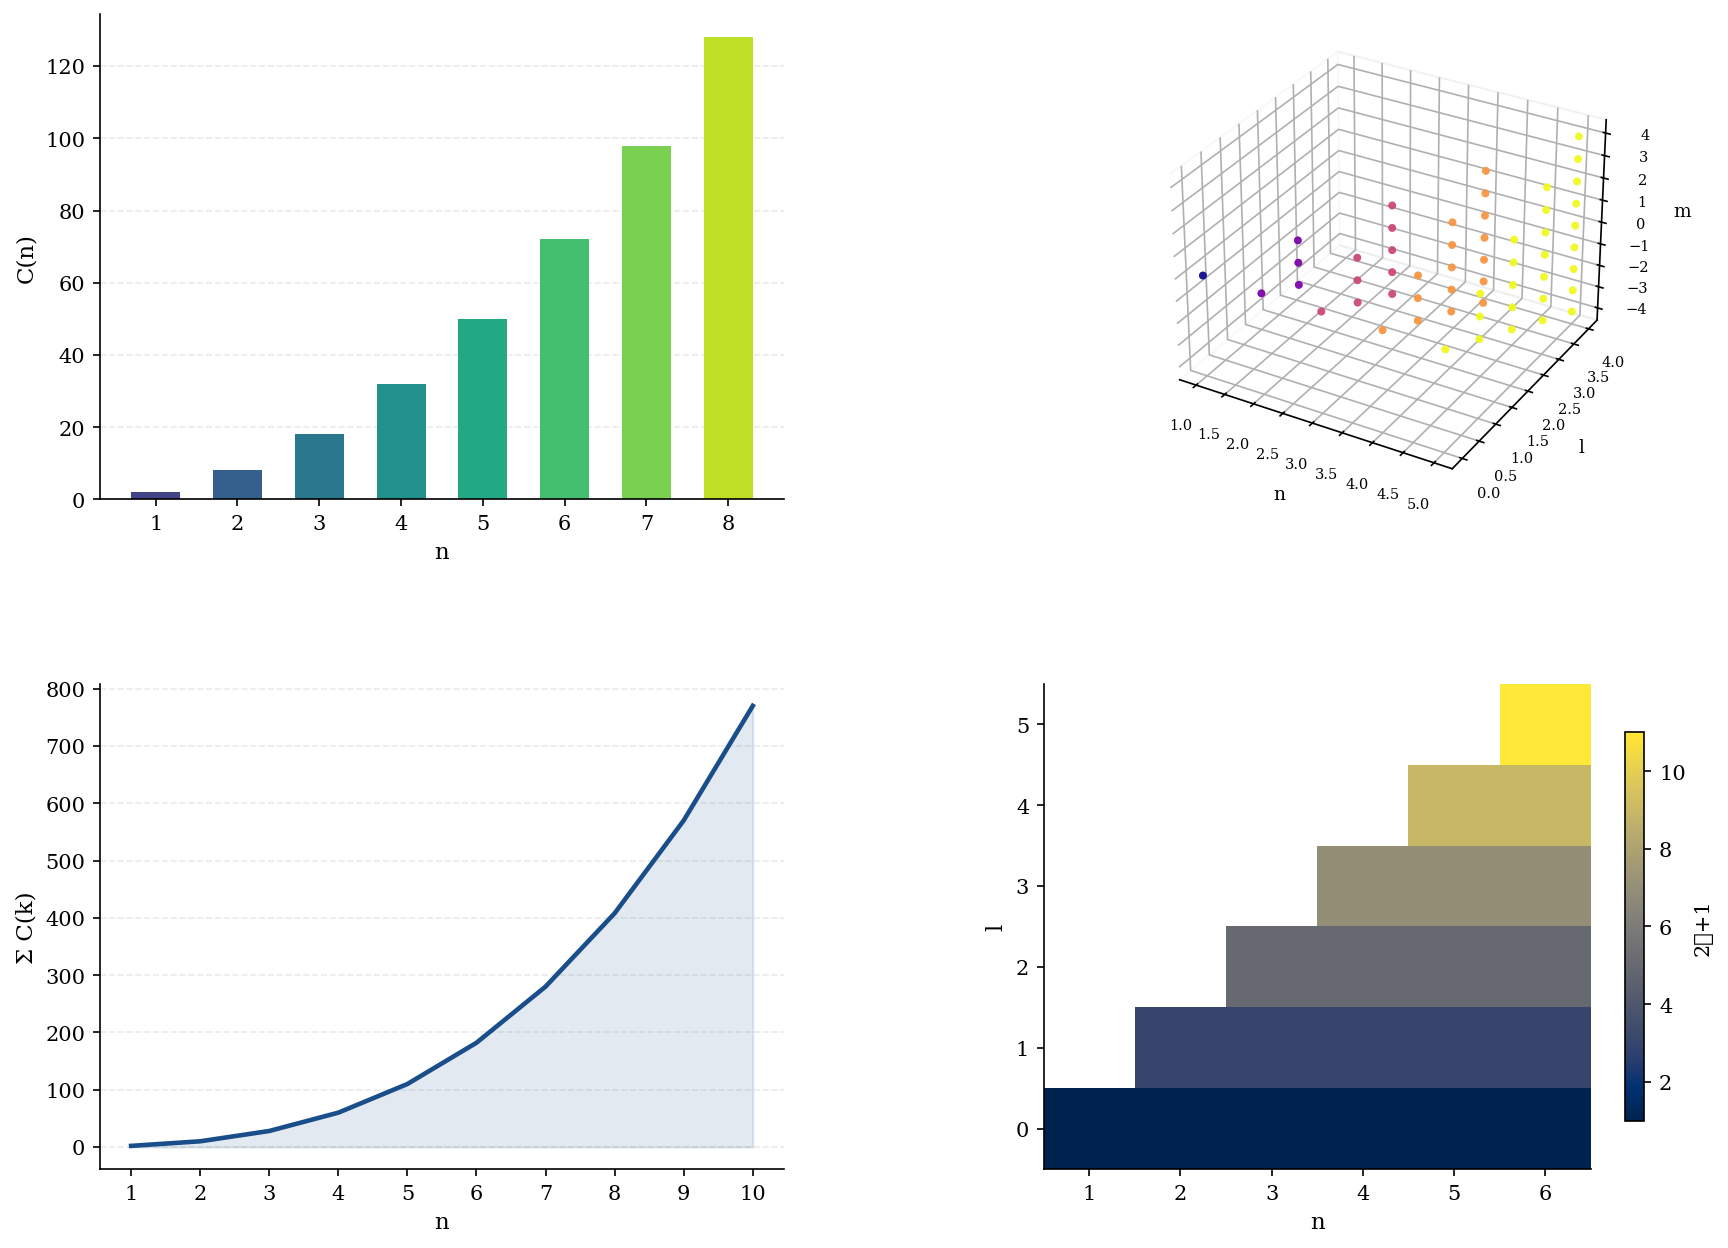
\includegraphics[width=\textwidth]{panel1_partition_geometry.png}
    \caption{\textbf{Partition Space Geometry.}
    (\textbf{A})~Shell capacity $C(n) = 2n^2$ for partition depths
    $n = 1, \ldots, 8$.  Each bar counts the number of valid coordinate
    quadruples $(\ell, m, s)$ at depth $n$: $\ell$ ranges over
    $\{0, \ldots, n-1\}$, $m$ over $\{-\ell, \ldots, +\ell\}$, and
    $s \in \{-\tfrac{1}{2}, +\tfrac{1}{2}\}$, giving
    $2\sum_{\ell=0}^{n-1}(2\ell+1) = 2n^2$ distinct addresses per shell.
    Bars are coloured from cool (shallow) to warm (deep) to indicate
    structural richness increasing with depth.
    (\textbf{B})~Three-dimensional scatter of all valid partition
    coordinates $(n, \ell, m)$ for $n \leq 5$, with spin parity $s$
    doubling each point's multiplicity.  Each point represents a unique
    node identity in the \srn\ network.  Depth $n$ determines the
    colour; the triangular cross-section at each depth reflects the
    constraint $|\,m\,| \leq \ell < n$.  The geometry is the discrete
    analogue of the hydrogen-atom orbital manifold arising from
    $\mathrm{SO}(3)$ representation theory.
    (\textbf{C})~Cumulative coordinate count
    $\sum_{k=1}^{n} 2k^2 = \tfrac{n(n+1)(2n+1)}{3}$ as a function of
    depth $n$.  By $n = 4$, the address space has $110$ distinct nodes;
    by $n = 6$, it reaches $182$.  The filled area emphasises the
    super-linear growth of the address space with depth.
    (\textbf{D})~Heatmap of the number of valid orientation indices
    $2\ell + 1$ over the $(n, \ell)$ grid for $n, \ell \in \{1,\ldots,6\}$.
    Grey (NaN) cells are structurally forbidden ($\ell \geq n$): they
    cannot be individuated at the given depth.  Permitted cells grow
    darker as $\ell$ increases, reflecting the widening orientation fan.
    The triangular forbidden region is the discrete shadow of the angular
    momentum constraint $\ell \in \{0, \ldots, n-1\}$.}
    \label{fig:panel1}
\end{figure*}

% ── Panel 2: Entropic Floor and Catalytic Dynamics ───────────────────────────

\begin{figure*}[!htbp]
    \centering
    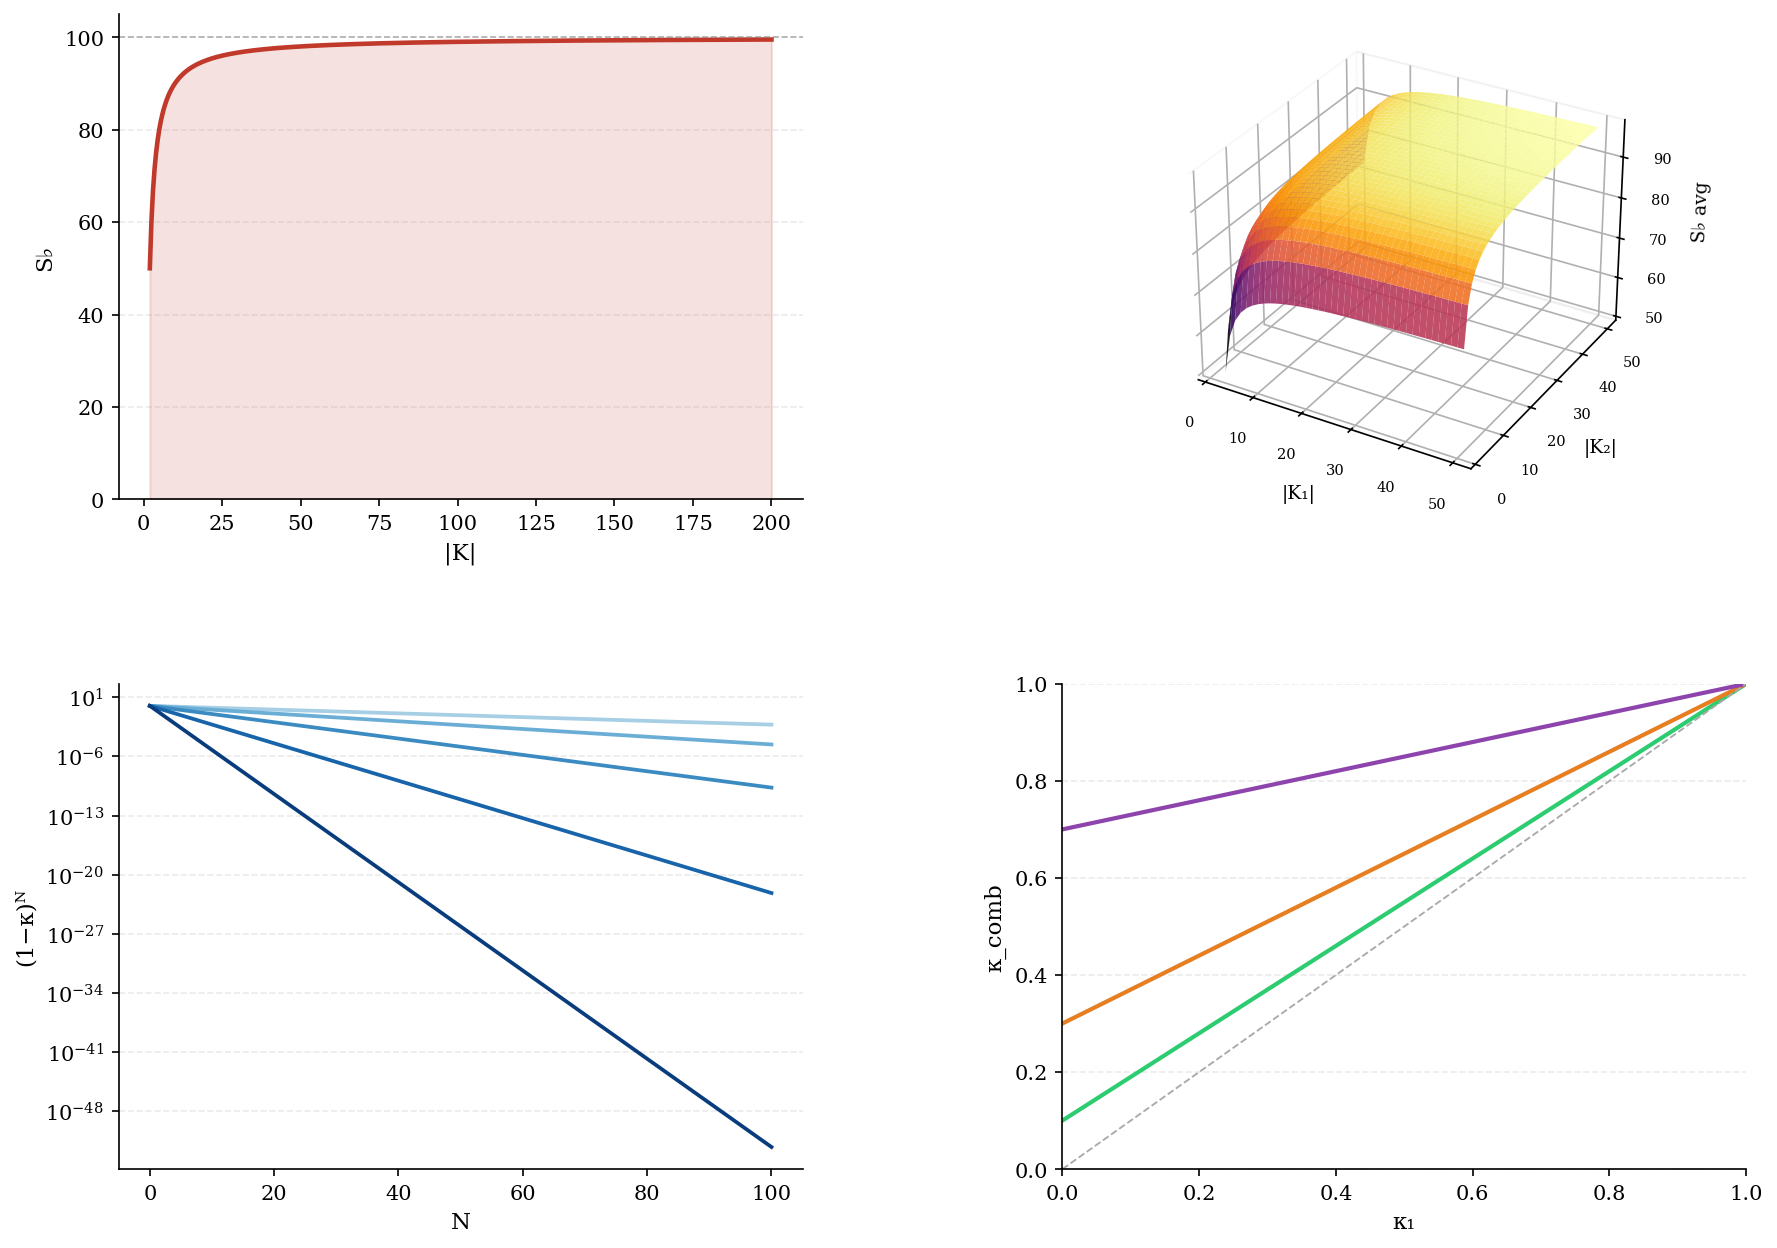
\includegraphics[width=\textwidth]{panel2_entropic_floor.png}
    \caption{\textbf{Entropic Floor and Catalytic Dynamics.}
    (\textbf{A})~The entropic floor $\floor(K) = 100(1 - 1/|K|)$ as a
    function of the receiver's knowledge framework size $|K|$, for
    $|K| \in [2, 200]$.  The filled region marks the range of
    achievable S-values.  The dashed line at $\floor = 100$ is the
    unattainable limit: perfect knowledge requires $|K| = \infty$.  At
    $|K| = 2$, the floor is $50$; at $|K| = 10$, it is $90$; at
    $|K| = 100$, it is $99$.  No finite receiver can close the gap to
    zero error, regardless of expression quality.
    (\textbf{B})~Three-dimensional surface of the average floor
    $\tfrac{1}{2}({\floor}(K_1) + {\floor}(K_2)) =
    50(2 - 1/|K_1| - 1/|K_2|)$ over two independent receiver sizes
    $|K_1|, |K_2| \in [2, 50]$.  The surface rises monotonically in both
    directions and remains strictly below $100$ everywhere.  The two
    receivers each contribute an independent positive floor; the average
    is the relevant quantity for cross-node evaluation, where neither
    receiver can achieve zero error in isolation.
    (\textbf{C})~Log-scale catalytic residual $(1-\kappa)^N$ as a
    function of step count $N \in [0, 100]$ for five catalyst strengths
    $\kappa \in \{0.05, 0.1, 0.2, 0.4, 0.7\}$ (light to dark).  All
    curves converge to zero, confirming the Borel-Cantelli analogue
    (Theorem~\ref{thm:catalyst}): repeated application of any catalyst
    with $\kappa > 0$ drives the residual to zero exponentially fast.
    The rate is $(1-\kappa)$ per step: a catalyst of strength $0.7$
    reduces the residual to $< 10^{-5}$ within $30$ steps; one of
    strength $0.05$ requires $\sim 200$ steps for the same reduction.
    (\textbf{D})~Composite catalytic power
    $\kappa_{\mathrm{comb}}(\kappa_1, \kappa_2)
    = 1 - (1 - \kappa_1)(1 - \kappa_2)$ as $\kappa_1$ varies over
    $[0,1]$ for three fixed values $\kappa_2 \in \{0.1, 0.3, 0.7\}$
    (green, orange, purple).  The diagonal reference line marks
    $\kappa_{\mathrm{comb}} = \kappa_1$.  Every curve lies strictly
    above the diagonal for $\kappa_1 \in (0,1)$, confirming that
    combining two catalysts always outperforms either alone.  A locally
    infeasible catalyst ($\kappa_2$ from a node where $S = 100$) retains
    positive composite power by the Miracle Principle
    (Corollary~\ref{cor:miracle}).}
    \label{fig:panel2}
\end{figure*}

% ── Panel 3: Composition Inflation ───────────────────────────────────────────

\begin{figure*}[!htbp]
    \centering
    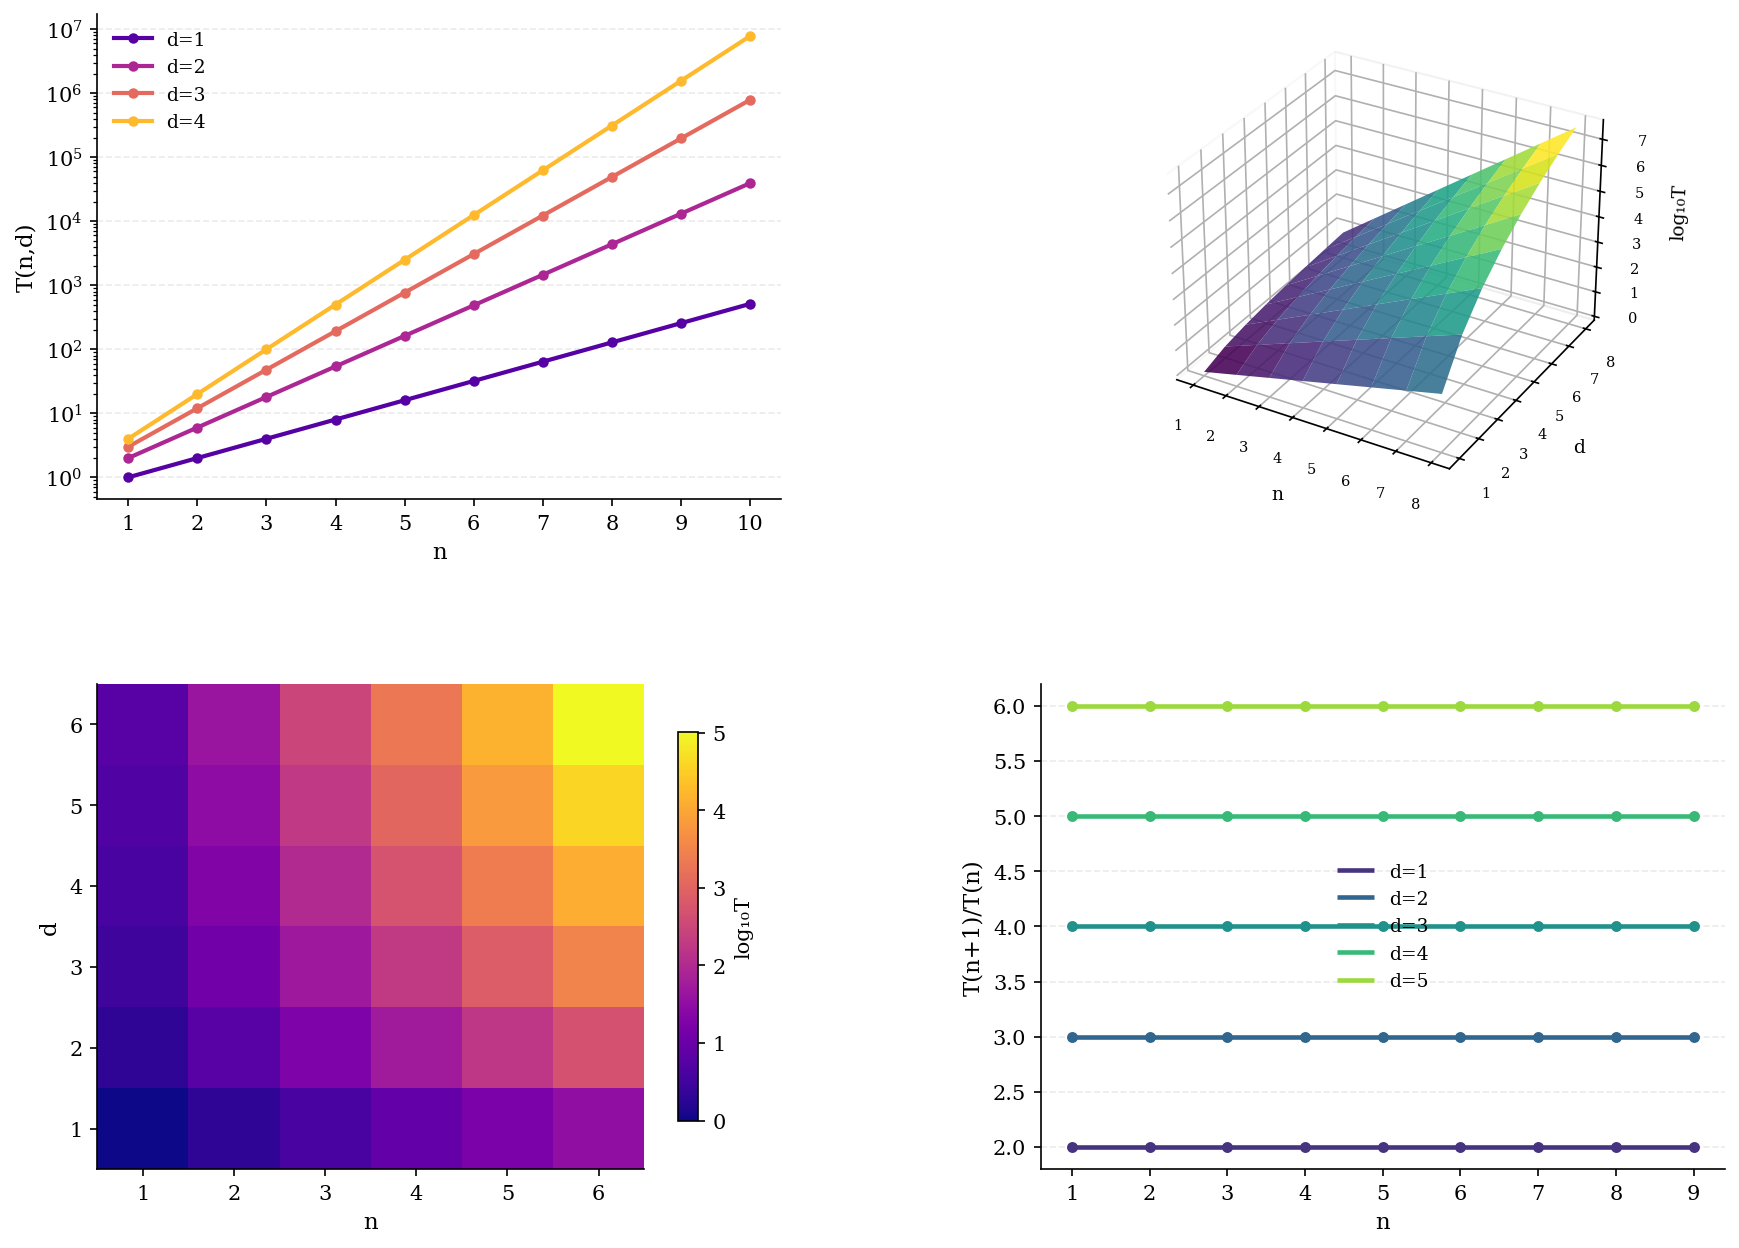
\includegraphics[width=\textwidth]{panel3_composition_inflation.png}
    \caption{\textbf{Composition Inflation $T(n,d) = d(1+d)^{n-1}$.}
    (\textbf{A})~Log-scale growth of $T(n,d)$ versus composition depth
    $n \in \{1, \ldots, 10\}$ for operator counts $d \in \{1, 2, 3, 4\}$.
    All curves are strictly exponential in $n$; the base $(1+d)$
    increases with $d$, so higher operator counts produce faster
    trajectory proliferation.  At $n = 10$ and $d = 4$, the number of
    distinguishable labeled trajectories exceeds $2 \times 10^6$.  The
    linear regime ($n = 1$, where $T = d$ regardless of base) is the
    unique fixed point visible at the left edge.
    (\textbf{B})~Three-dimensional surface of $\log_{10} T(n,d)$ over
    $(n, d) \in \{1, \ldots, 8\}^2$.  The surface is coloured by height:
    cool shades indicate few trajectories; warm shades indicate many.
    The exponential dependence on $n$ and the linear-then-exponential
    dependence on $d$ produce a surface that rises steeply in both
    directions, but more steeply along $n$ for fixed $d > 1$.
    (\textbf{C})~Heatmap of $\log_{10} T(n,d)$ for
    $(n, d) \in \{1,\ldots,6\}^2$.  Each cell is coloured by the
    base-10 logarithm of the trajectory count.  The heatmap reveals
    the multiplicative structure: moving one step right (increasing $n$
    by $1$) multiplies $T$ by $(1+d)$; moving one step up (increasing
    $d$ by $1$) adds an additional factor that varies with $n$.  The
    fastest-growing cell at $(n=6, d=6)$ has $T = 6 \cdot 7^5 \approx
    7 \times 10^4$ trajectories.
    (\textbf{D})~Growth ratio $T(n+1, d) / T(n, d) = 1 + d$ as a
    function of $n$ for $d \in \{1, 2, 3, 4, 5\}$.  Each curve is a
    horizontal line, confirming that the ratio is exactly constant in
    $n$: the exponential base $(1+d)$ is independent of depth.  This
    is a structural consequence of the binomial identity underlying the
    Composition Inflation theorem (Theorem~\ref{thm:inflation}), not
    a numerical accident.  Dots mark the integer values of $n$ where
    the ratio was evaluated.}
    \label{fig:panel3}
\end{figure*}

% ── Panel 4: Forest Dynamics and Receiver-Relative Evaluation ────────────────

\begin{figure*}[!htbp]
    \centering
    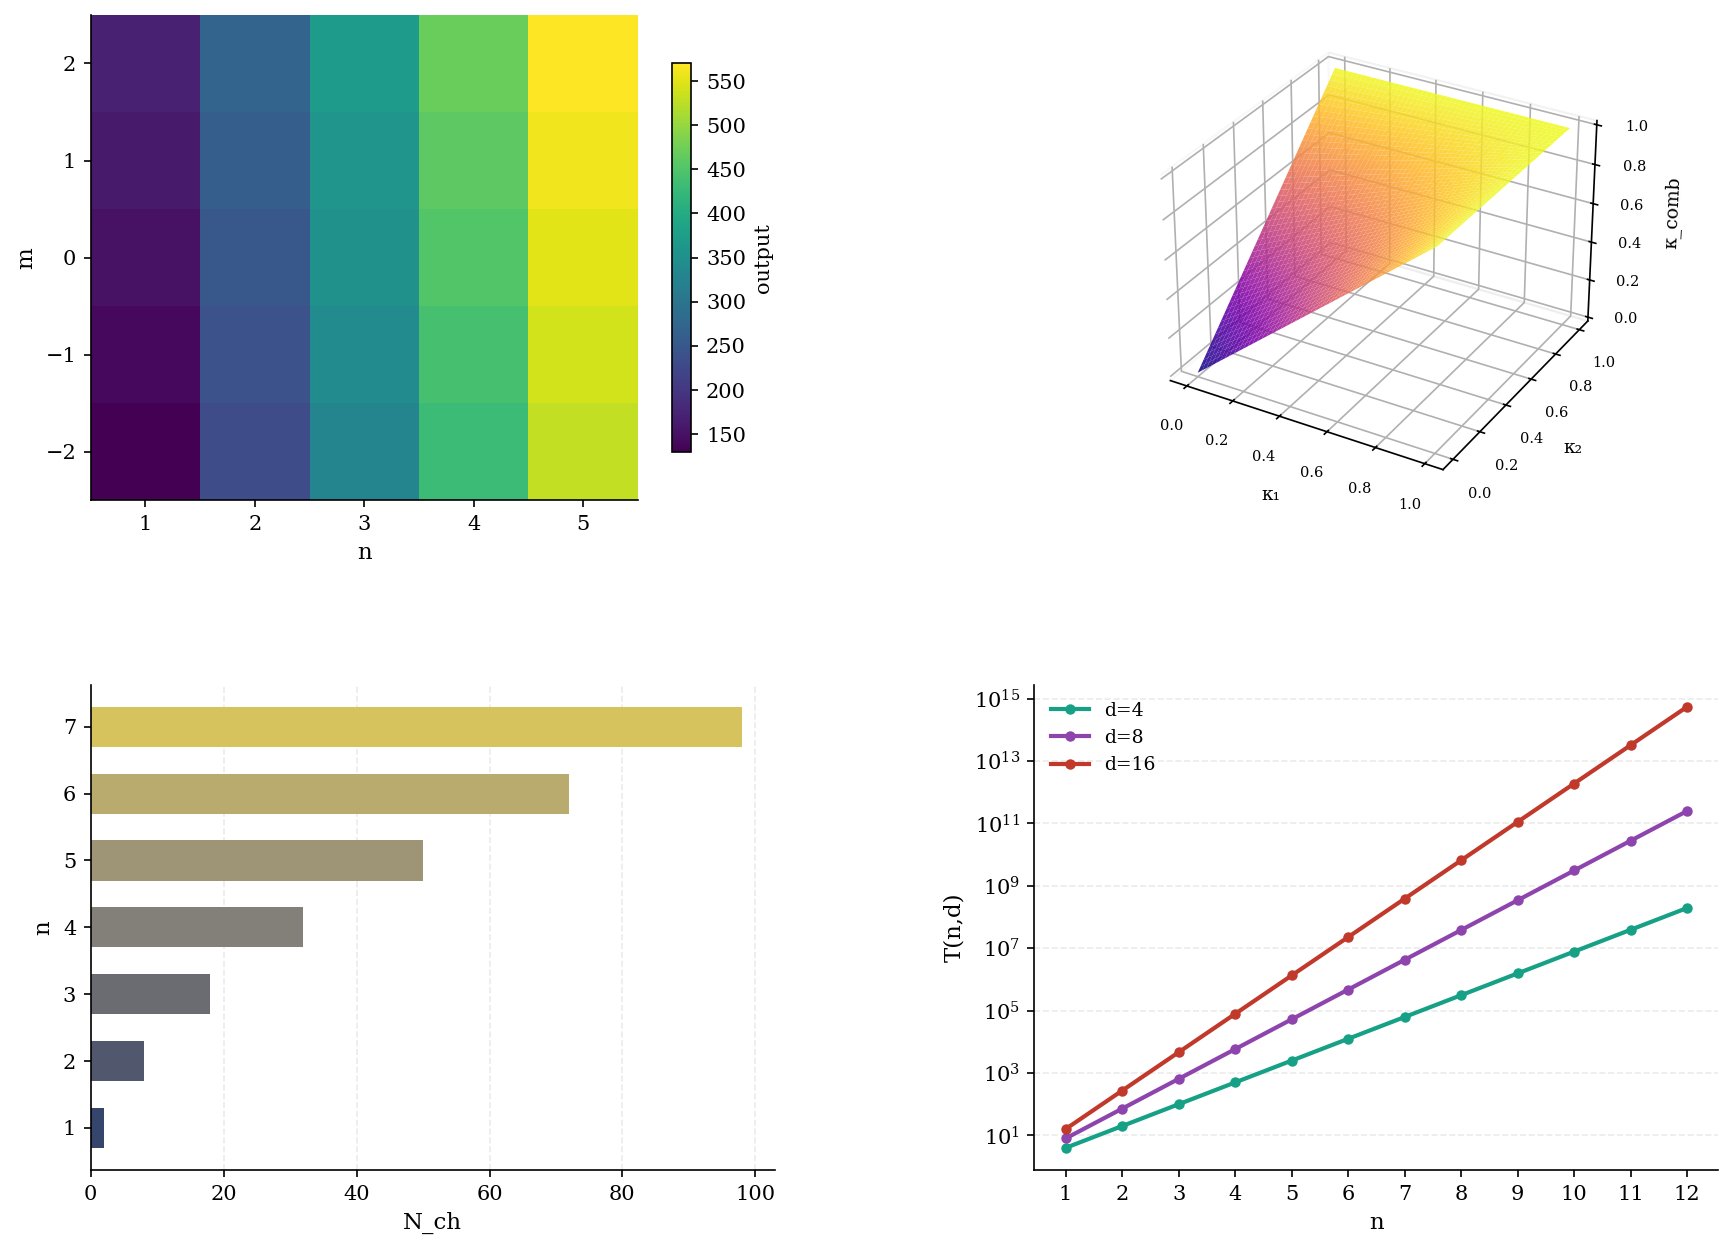
\includegraphics[width=\textwidth]{panel4_forest_dynamics.png}
    \caption{\textbf{Forest Dynamics and Receiver-Relative Evaluation.}
    (\textbf{A})~Heatmap of the receiver-relative output
    $v = 100n + 10m + M$ (with partition count $M = 50$ fixed)
    across the $(n, m)$ node grid, $n \in \{1,\ldots,5\}$,
    $m \in \{-2,-1,0,+1,+2\}$.  Every cell yields a distinct value:
    no two nodes evaluate the same expression to the same result.
    This is a direct numerical illustration of
    Theorem~\ref{thm:rr} (Receiver-Relativity): the same \srn\
    expression produces different output at every node in the network,
    with all outputs simultaneously valid.  The colour gradient
    encodes the output value; no central authority reconciles the
    divergent results.
    (\textbf{B})~Three-dimensional surface of composite catalytic power
    $\kappa_{\mathrm{comb}}(\kappa_1, \kappa_2)
    = 1 - (1 - \kappa_1)(1 - \kappa_2)$ over $(\kappa_1, \kappa_2)
    \in [0,1]^2$.  The surface is bounded in $[0,1]^2$, rises
    monotonically in both arguments, and reaches $1$ only at the corner
    $(\kappa_1, \kappa_2) = (1, 1)$.  The curvature of the surface
    reflects the multiplicative—not additive—structure of catalytic
    combination: a second catalyst of strength $\kappa_2$ acts on the
    \emph{residual} $1 - \kappa_1$, not on the full domain.
    (\textbf{C})~Forced channel count $N_{\mathrm{ch}} = 2n^2$ per
    partition depth $n \in \{1,\ldots,7\}$, shown as horizontal bars.
    These are the independent communication channels structurally
    mandated by the node's topology (Theorem~\ref{thm:channels}): a
    node at depth $4$ must support $32$ independent channels; at depth
    $7$, it must support $98$.  The channel count is not a design
    parameter; it is forced by the cycle rank of the contact graph on
    the shell elements.  Bars are coloured by depth.
    (\textbf{D})~Trajectory encoding capacity $T(n, d)$ for channel
    counts $d \in \{4, 8, 16\}$ and composition depths $n = 1,\ldots,12$,
    on a log scale.  Each curve represents the number of distinguishable
    \srn\ expressions encodable as timing trajectories at that channel
    count.  At $n = 12$ and $d = 16$, the capacity reaches
    $T = 16 \cdot 17^{11} \approx 3.4 \times 10^{13}$ distinct
    expressions.  The channel count $d = 4$ corresponds to a minimal
    four-channel node (depth $n = 1$, $N_{\mathrm{ch}} = 2$); $d = 16$
    corresponds to a depth-$3$ node ($N_{\mathrm{ch}} = 18$).  Existing
    internet infrastructure, which already measures timing deviations
    $\Delta P(k)$ at nanosecond resolution across multiple channels,
    operates comfortably in this regime.}
    \label{fig:panel4}
\end{figure*}
.
% ============================================================

% ── Panel 1: Partition Space Geometry ────────────────────────────────────────

\begin{figure*}[!htbp]
    \centering
    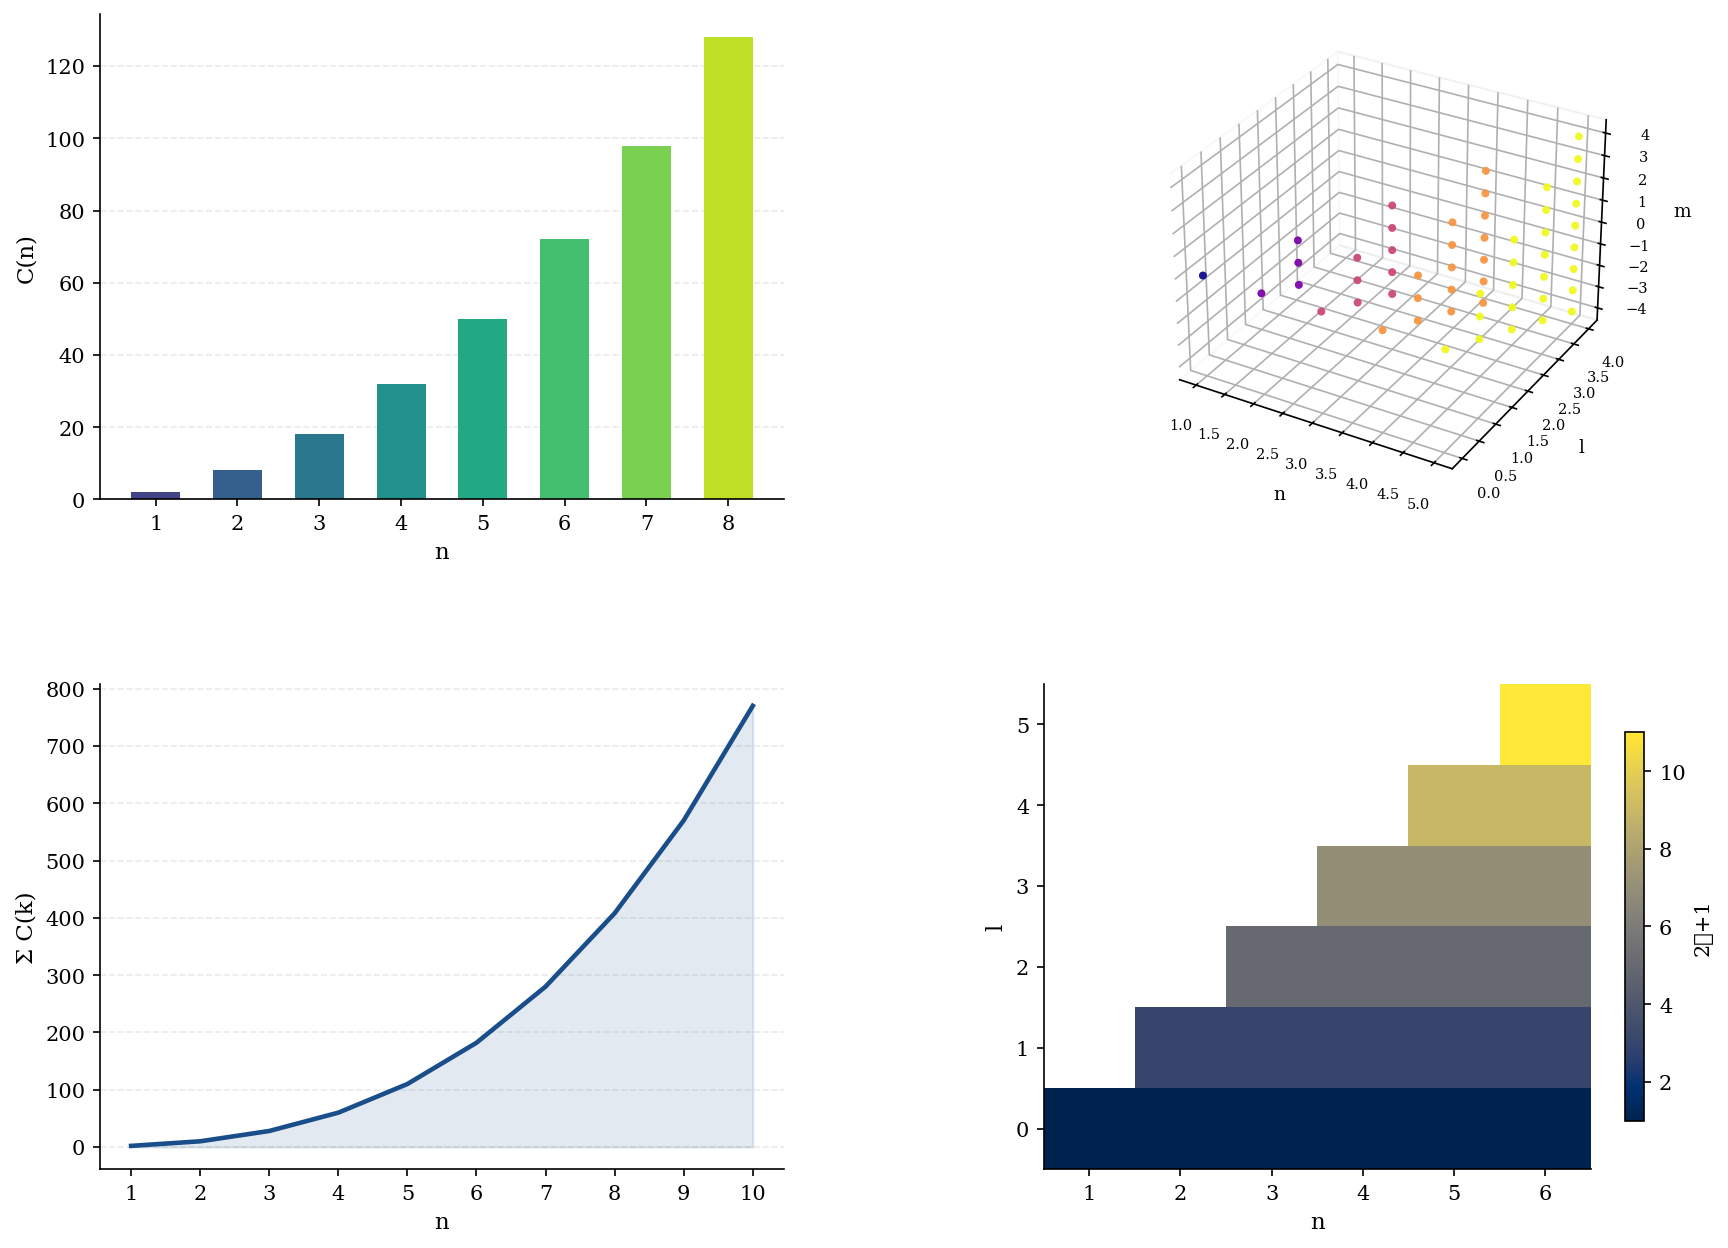
\includegraphics[width=\textwidth]{panel1_partition_geometry.png}
    \caption{\textbf{Partition Space Geometry.}
    (\textbf{A})~Shell capacity $C(n) = 2n^2$ for partition depths
    $n = 1, \ldots, 8$.  Each bar counts the number of valid coordinate
    quadruples $(\ell, m, s)$ at depth $n$: $\ell$ ranges over
    $\{0, \ldots, n-1\}$, $m$ over $\{-\ell, \ldots, +\ell\}$, and
    $s \in \{-\tfrac{1}{2}, +\tfrac{1}{2}\}$, giving
    $2\sum_{\ell=0}^{n-1}(2\ell+1) = 2n^2$ distinct addresses per shell.
    Bars are coloured from cool (shallow) to warm (deep) to indicate
    structural richness increasing with depth.
    (\textbf{B})~Three-dimensional scatter of all valid partition
    coordinates $(n, \ell, m)$ for $n \leq 5$, with spin parity $s$
    doubling each point's multiplicity.  Each point represents a unique
    node identity in the \srn\ network.  Depth $n$ determines the
    colour; the triangular cross-section at each depth reflects the
    constraint $|\,m\,| \leq \ell < n$.  The geometry is the discrete
    analogue of the hydrogen-atom orbital manifold arising from
    $\mathrm{SO}(3)$ representation theory.
    (\textbf{C})~Cumulative coordinate count
    $\sum_{k=1}^{n} 2k^2 = \tfrac{n(n+1)(2n+1)}{3}$ as a function of
    depth $n$.  By $n = 4$, the address space has $110$ distinct nodes;
    by $n = 6$, it reaches $182$.  The filled area emphasises the
    super-linear growth of the address space with depth.
    (\textbf{D})~Heatmap of the number of valid orientation indices
    $2\ell + 1$ over the $(n, \ell)$ grid for $n, \ell \in \{1,\ldots,6\}$.
    Grey (NaN) cells are structurally forbidden ($\ell \geq n$): they
    cannot be individuated at the given depth.  Permitted cells grow
    darker as $\ell$ increases, reflecting the widening orientation fan.
    The triangular forbidden region is the discrete shadow of the angular
    momentum constraint $\ell \in \{0, \ldots, n-1\}$.}
    \label{fig:panel1}
\end{figure*}

% ── Panel 2: Entropic Floor and Catalytic Dynamics ───────────────────────────

\begin{figure*}[!htbp]
    \centering
    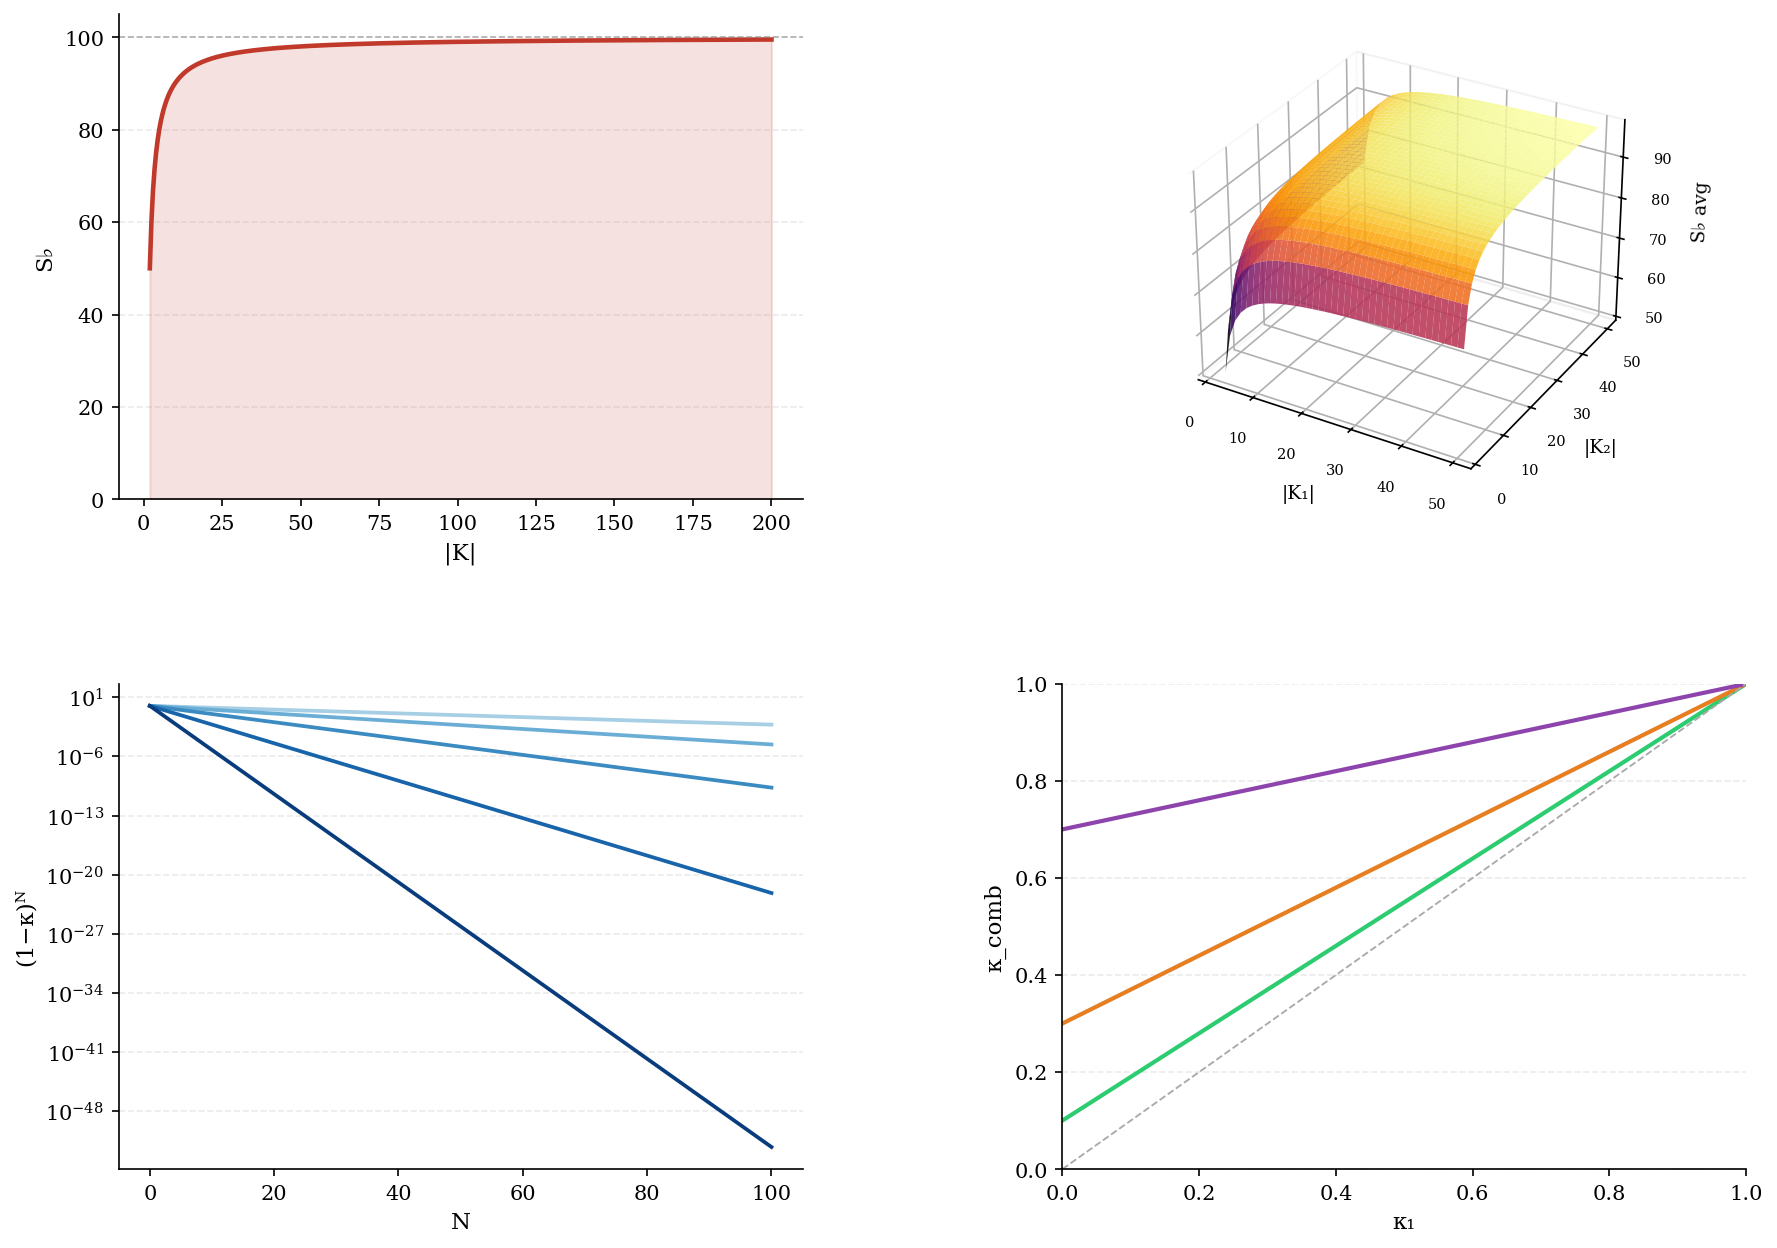
\includegraphics[width=\textwidth]{panel2_entropic_floor.png}
    \caption{\textbf{Entropic Floor and Catalytic Dynamics.}
    (\textbf{A})~The entropic floor $\floor(K) = 100(1 - 1/|K|)$ as a
    function of the receiver's knowledge framework size $|K|$, for
    $|K| \in [2, 200]$.  The filled region marks the range of
    achievable S-values.  The dashed line at $\floor = 100$ is the
    unattainable limit: perfect knowledge requires $|K| = \infty$.  At
    $|K| = 2$, the floor is $50$; at $|K| = 10$, it is $90$; at
    $|K| = 100$, it is $99$.  No finite receiver can close the gap to
    zero error, regardless of expression quality.
    (\textbf{B})~Three-dimensional surface of the average floor
    $\tfrac{1}{2}({\floor}(K_1) + {\floor}(K_2)) =
    50(2 - 1/|K_1| - 1/|K_2|)$ over two independent receiver sizes
    $|K_1|, |K_2| \in [2, 50]$.  The surface rises monotonically in both
    directions and remains strictly below $100$ everywhere.  The two
    receivers each contribute an independent positive floor; the average
    is the relevant quantity for cross-node evaluation, where neither
    receiver can achieve zero error in isolation.
    (\textbf{C})~Log-scale catalytic residual $(1-\kappa)^N$ as a
    function of step count $N \in [0, 100]$ for five catalyst strengths
    $\kappa \in \{0.05, 0.1, 0.2, 0.4, 0.7\}$ (light to dark).  All
    curves converge to zero, confirming the Borel-Cantelli analogue
    (Theorem~\ref{thm:catalyst}): repeated application of any catalyst
    with $\kappa > 0$ drives the residual to zero exponentially fast.
    The rate is $(1-\kappa)$ per step: a catalyst of strength $0.7$
    reduces the residual to $< 10^{-5}$ within $30$ steps; one of
    strength $0.05$ requires $\sim 200$ steps for the same reduction.
    (\textbf{D})~Composite catalytic power
    $\kappa_{\mathrm{comb}}(\kappa_1, \kappa_2)
    = 1 - (1 - \kappa_1)(1 - \kappa_2)$ as $\kappa_1$ varies over
    $[0,1]$ for three fixed values $\kappa_2 \in \{0.1, 0.3, 0.7\}$
    (green, orange, purple).  The diagonal reference line marks
    $\kappa_{\mathrm{comb}} = \kappa_1$.  Every curve lies strictly
    above the diagonal for $\kappa_1 \in (0,1)$, confirming that
    combining two catalysts always outperforms either alone.  A locally
    infeasible catalyst ($\kappa_2$ from a node where $S = 100$) retains
    positive composite power by the Miracle Principle
    (Corollary~\ref{cor:miracle}).}
    \label{fig:panel2}
\end{figure*}

% ── Panel 3: Composition Inflation ───────────────────────────────────────────

\begin{figure*}[!htbp]
    \centering
    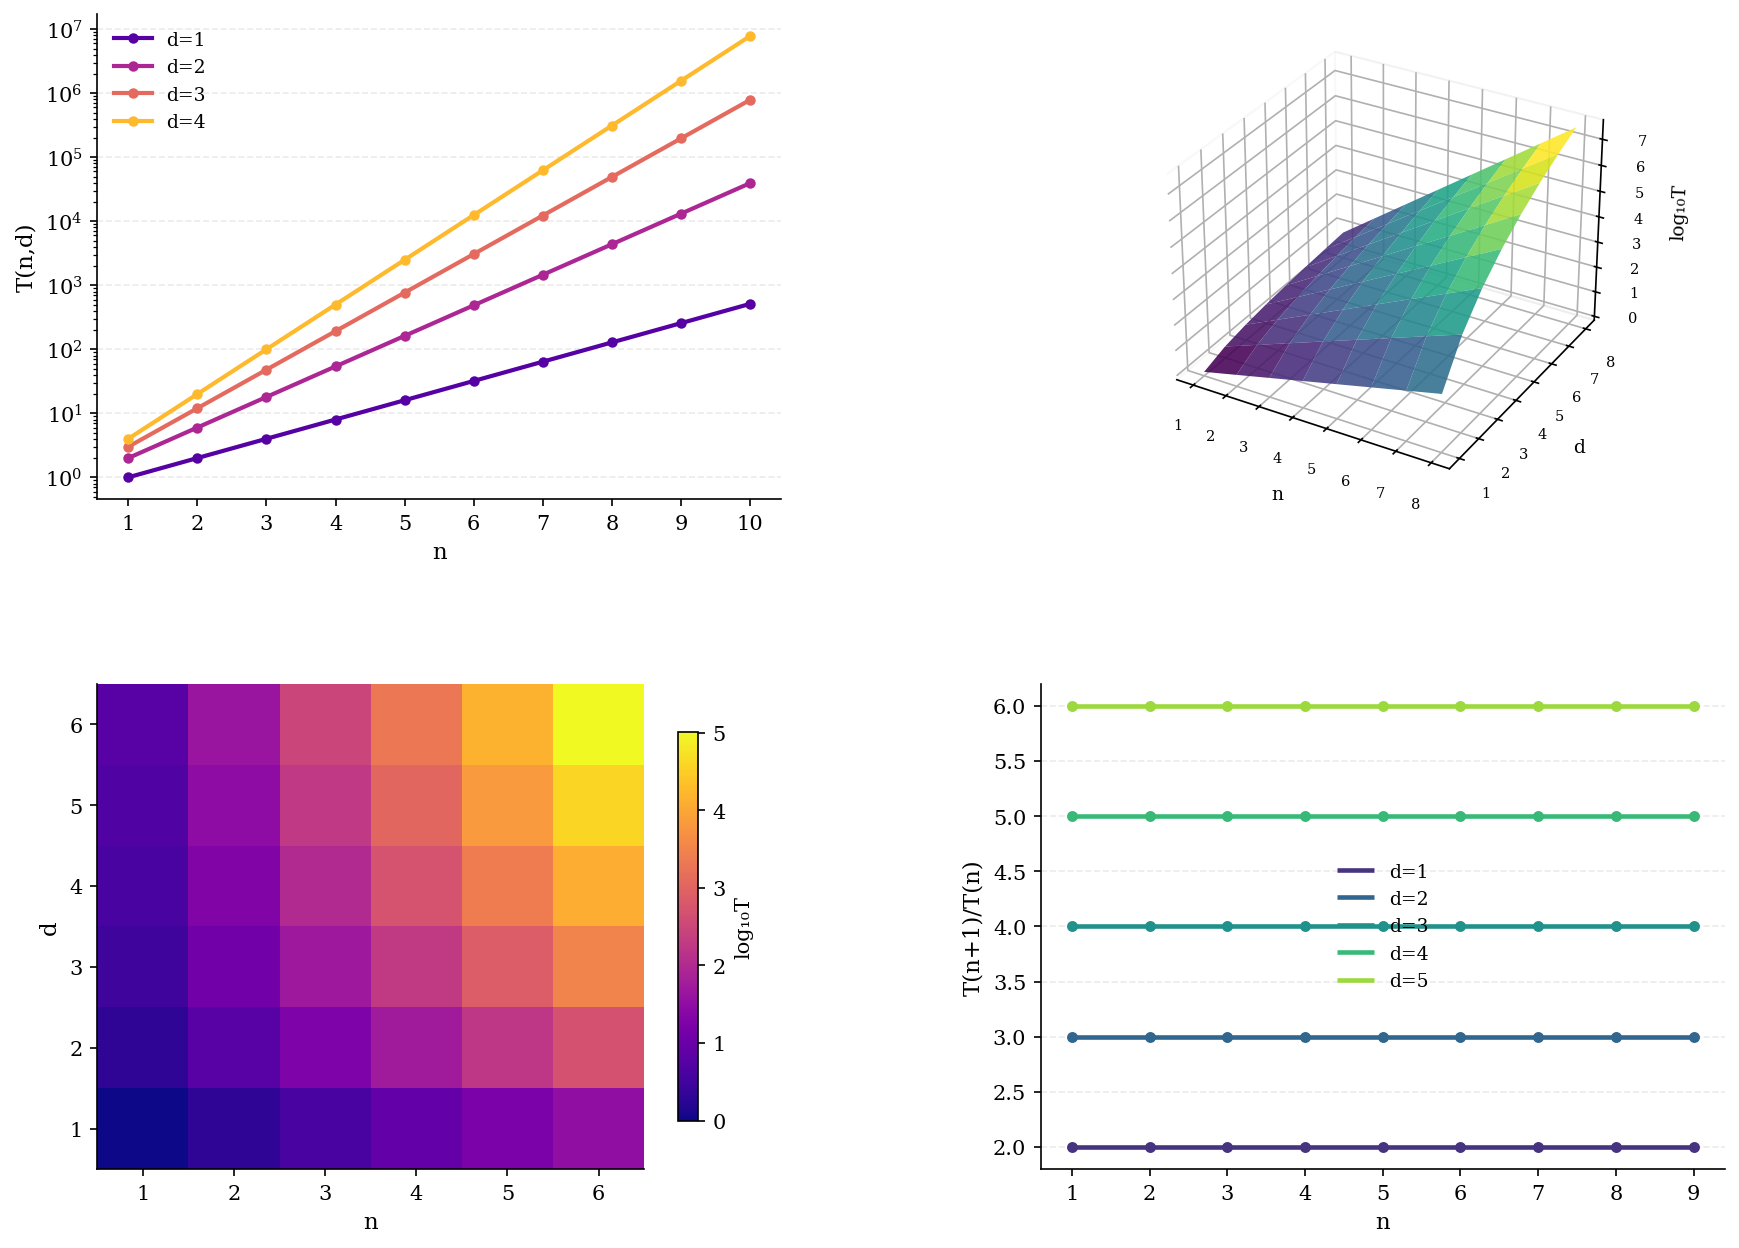
\includegraphics[width=\textwidth]{panel3_composition_inflation.png}
    \caption{\textbf{Composition Inflation $T(n,d) = d(1+d)^{n-1}$.}
    (\textbf{A})~Log-scale growth of $T(n,d)$ versus composition depth
    $n \in \{1, \ldots, 10\}$ for operator counts $d \in \{1, 2, 3, 4\}$.
    All curves are strictly exponential in $n$; the base $(1+d)$
    increases with $d$, so higher operator counts produce faster
    trajectory proliferation.  At $n = 10$ and $d = 4$, the number of
    distinguishable labeled trajectories exceeds $2 \times 10^6$.  The
    linear regime ($n = 1$, where $T = d$ regardless of base) is the
    unique fixed point visible at the left edge.
    (\textbf{B})~Three-dimensional surface of $\log_{10} T(n,d)$ over
    $(n, d) \in \{1, \ldots, 8\}^2$.  The surface is coloured by height:
    cool shades indicate few trajectories; warm shades indicate many.
    The exponential dependence on $n$ and the linear-then-exponential
    dependence on $d$ produce a surface that rises steeply in both
    directions, but more steeply along $n$ for fixed $d > 1$.
    (\textbf{C})~Heatmap of $\log_{10} T(n,d)$ for
    $(n, d) \in \{1,\ldots,6\}^2$.  Each cell is coloured by the
    base-10 logarithm of the trajectory count.  The heatmap reveals
    the multiplicative structure: moving one step right (increasing $n$
    by $1$) multiplies $T$ by $(1+d)$; moving one step up (increasing
    $d$ by $1$) adds an additional factor that varies with $n$.  The
    fastest-growing cell at $(n=6, d=6)$ has $T = 6 \cdot 7^5 \approx
    7 \times 10^4$ trajectories.
    (\textbf{D})~Growth ratio $T(n+1, d) / T(n, d) = 1 + d$ as a
    function of $n$ for $d \in \{1, 2, 3, 4, 5\}$.  Each curve is a
    horizontal line, confirming that the ratio is exactly constant in
    $n$: the exponential base $(1+d)$ is independent of depth.  This
    is a structural consequence of the binomial identity underlying the
    Composition Inflation theorem (Theorem~\ref{thm:inflation}), not
    a numerical accident.  Dots mark the integer values of $n$ where
    the ratio was evaluated.}
    \label{fig:panel3}
\end{figure*}

% ── Panel 4: Forest Dynamics and Receiver-Relative Evaluation ────────────────

\begin{figure*}[!htbp]
    \centering
    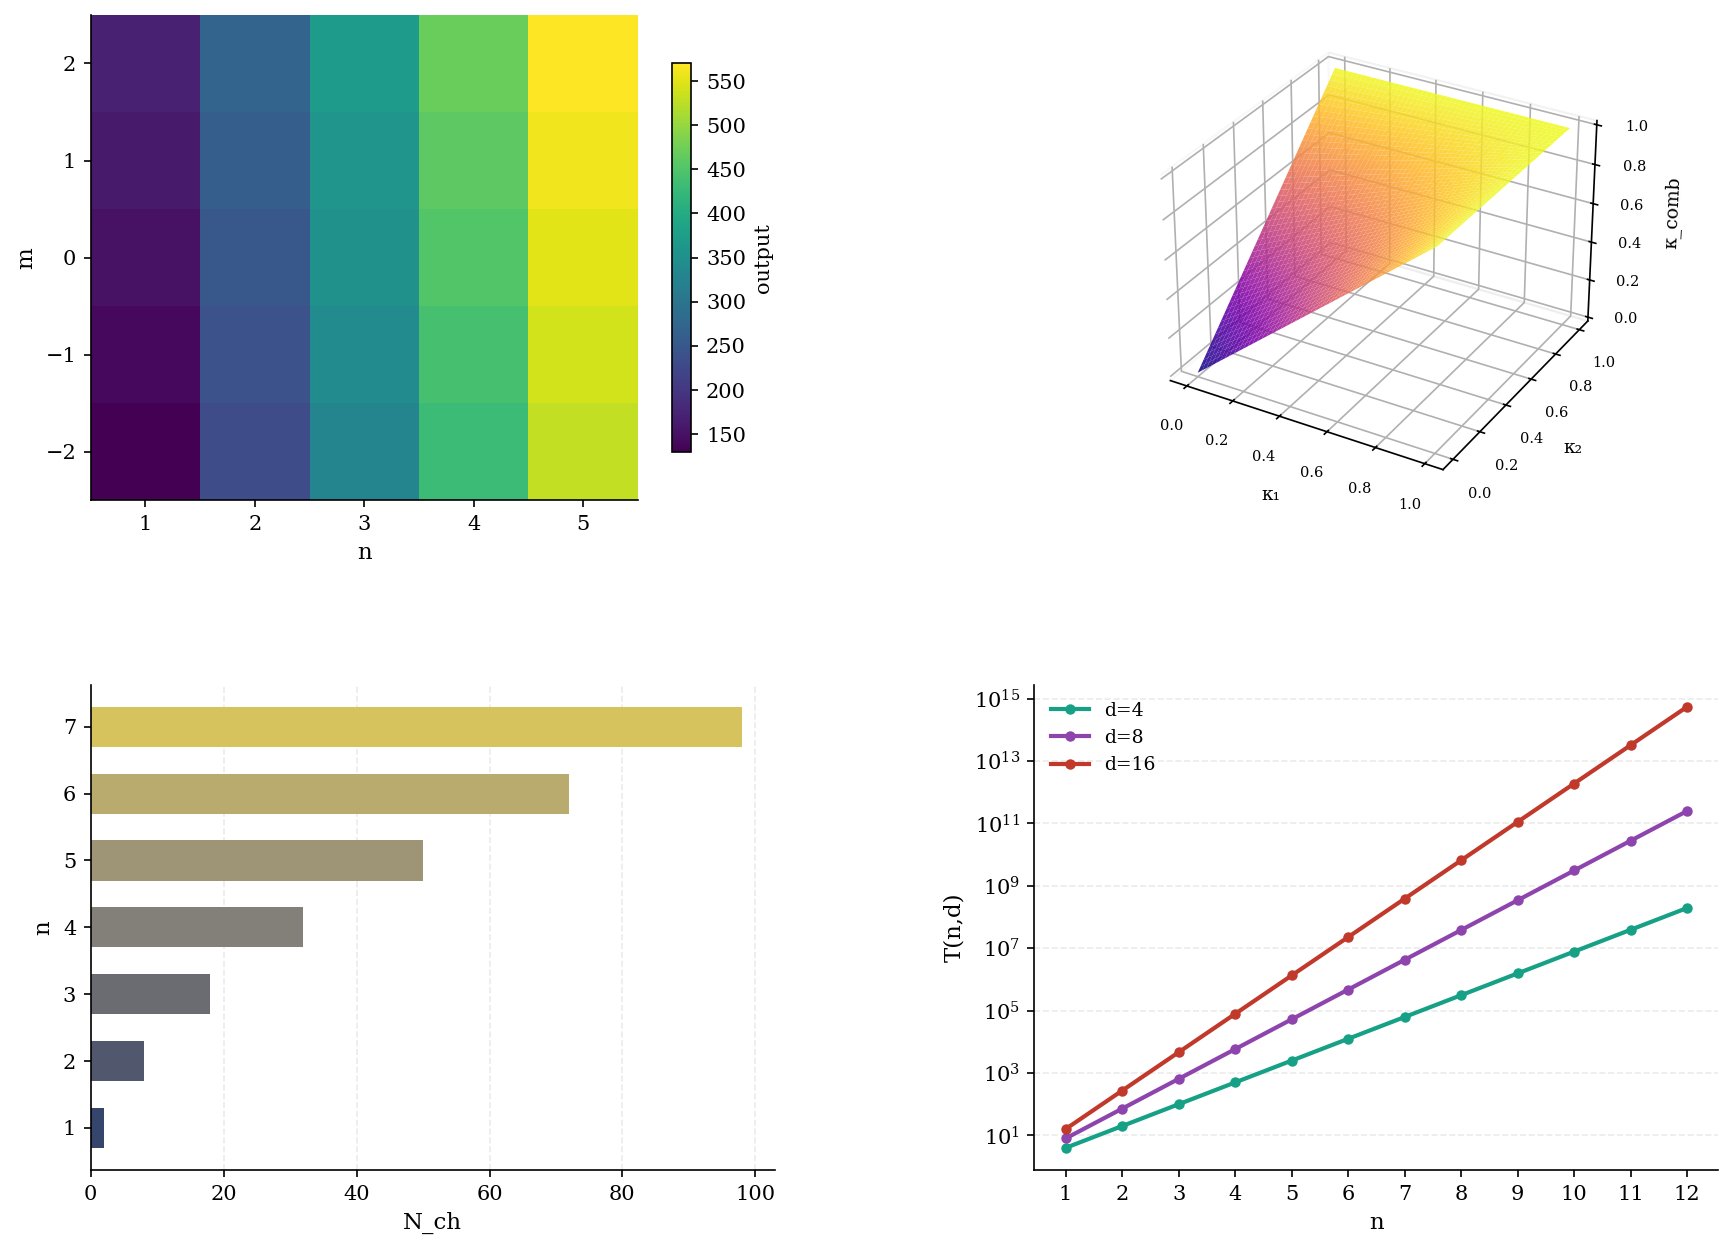
\includegraphics[width=\textwidth]{panel4_forest_dynamics.png}
    \caption{\textbf{Forest Dynamics and Receiver-Relative Evaluation.}
    (\textbf{A})~Heatmap of the receiver-relative output
    $v = 100n + 10m + M$ (with partition count $M = 50$ fixed)
    across the $(n, m)$ node grid, $n \in \{1,\ldots,5\}$,
    $m \in \{-2,-1,0,+1,+2\}$.  Every cell yields a distinct value:
    no two nodes evaluate the same expression to the same result.
    This is a direct numerical illustration of
    Theorem~\ref{thm:rr} (Receiver-Relativity): the same \srn\
    expression produces different output at every node in the network,
    with all outputs simultaneously valid.  The colour gradient
    encodes the output value; no central authority reconciles the
    divergent results.
    (\textbf{B})~Three-dimensional surface of composite catalytic power
    $\kappa_{\mathrm{comb}}(\kappa_1, \kappa_2)
    = 1 - (1 - \kappa_1)(1 - \kappa_2)$ over $(\kappa_1, \kappa_2)
    \in [0,1]^2$.  The surface is bounded in $[0,1]^2$, rises
    monotonically in both arguments, and reaches $1$ only at the corner
    $(\kappa_1, \kappa_2) = (1, 1)$.  The curvature of the surface
    reflects the multiplicative—not additive—structure of catalytic
    combination: a second catalyst of strength $\kappa_2$ acts on the
    \emph{residual} $1 - \kappa_1$, not on the full domain.
    (\textbf{C})~Forced channel count $N_{\mathrm{ch}} = 2n^2$ per
    partition depth $n \in \{1,\ldots,7\}$, shown as horizontal bars.
    These are the independent communication channels structurally
    mandated by the node's topology (Theorem~\ref{thm:channels}): a
    node at depth $4$ must support $32$ independent channels; at depth
    $7$, it must support $98$.  The channel count is not a design
    parameter; it is forced by the cycle rank of the contact graph on
    the shell elements.  Bars are coloured by depth.
    (\textbf{D})~Trajectory encoding capacity $T(n, d)$ for channel
    counts $d \in \{4, 8, 16\}$ and composition depths $n = 1,\ldots,12$,
    on a log scale.  Each curve represents the number of distinguishable
    \srn\ expressions encodable as timing trajectories at that channel
    count.  At $n = 12$ and $d = 16$, the capacity reaches
    $T = 16 \cdot 17^{11} \approx 3.4 \times 10^{13}$ distinct
    expressions.  The channel count $d = 4$ corresponds to a minimal
    four-channel node (depth $n = 1$, $N_{\mathrm{ch}} = 2$); $d = 16$
    corresponds to a depth-$3$ node ($N_{\mathrm{ch}} = 18$).  Existing
    internet infrastructure, which already measures timing deviations
    $\Delta P(k)$ at nanosecond resolution across multiple channels,
    operates comfortably in this regime.}
    \label{fig:panel4}
\end{figure*}
.
% ============================================================

% ── Panel 1: Partition Space Geometry ────────────────────────────────────────

\begin{figure*}[!htbp]
    \centering
    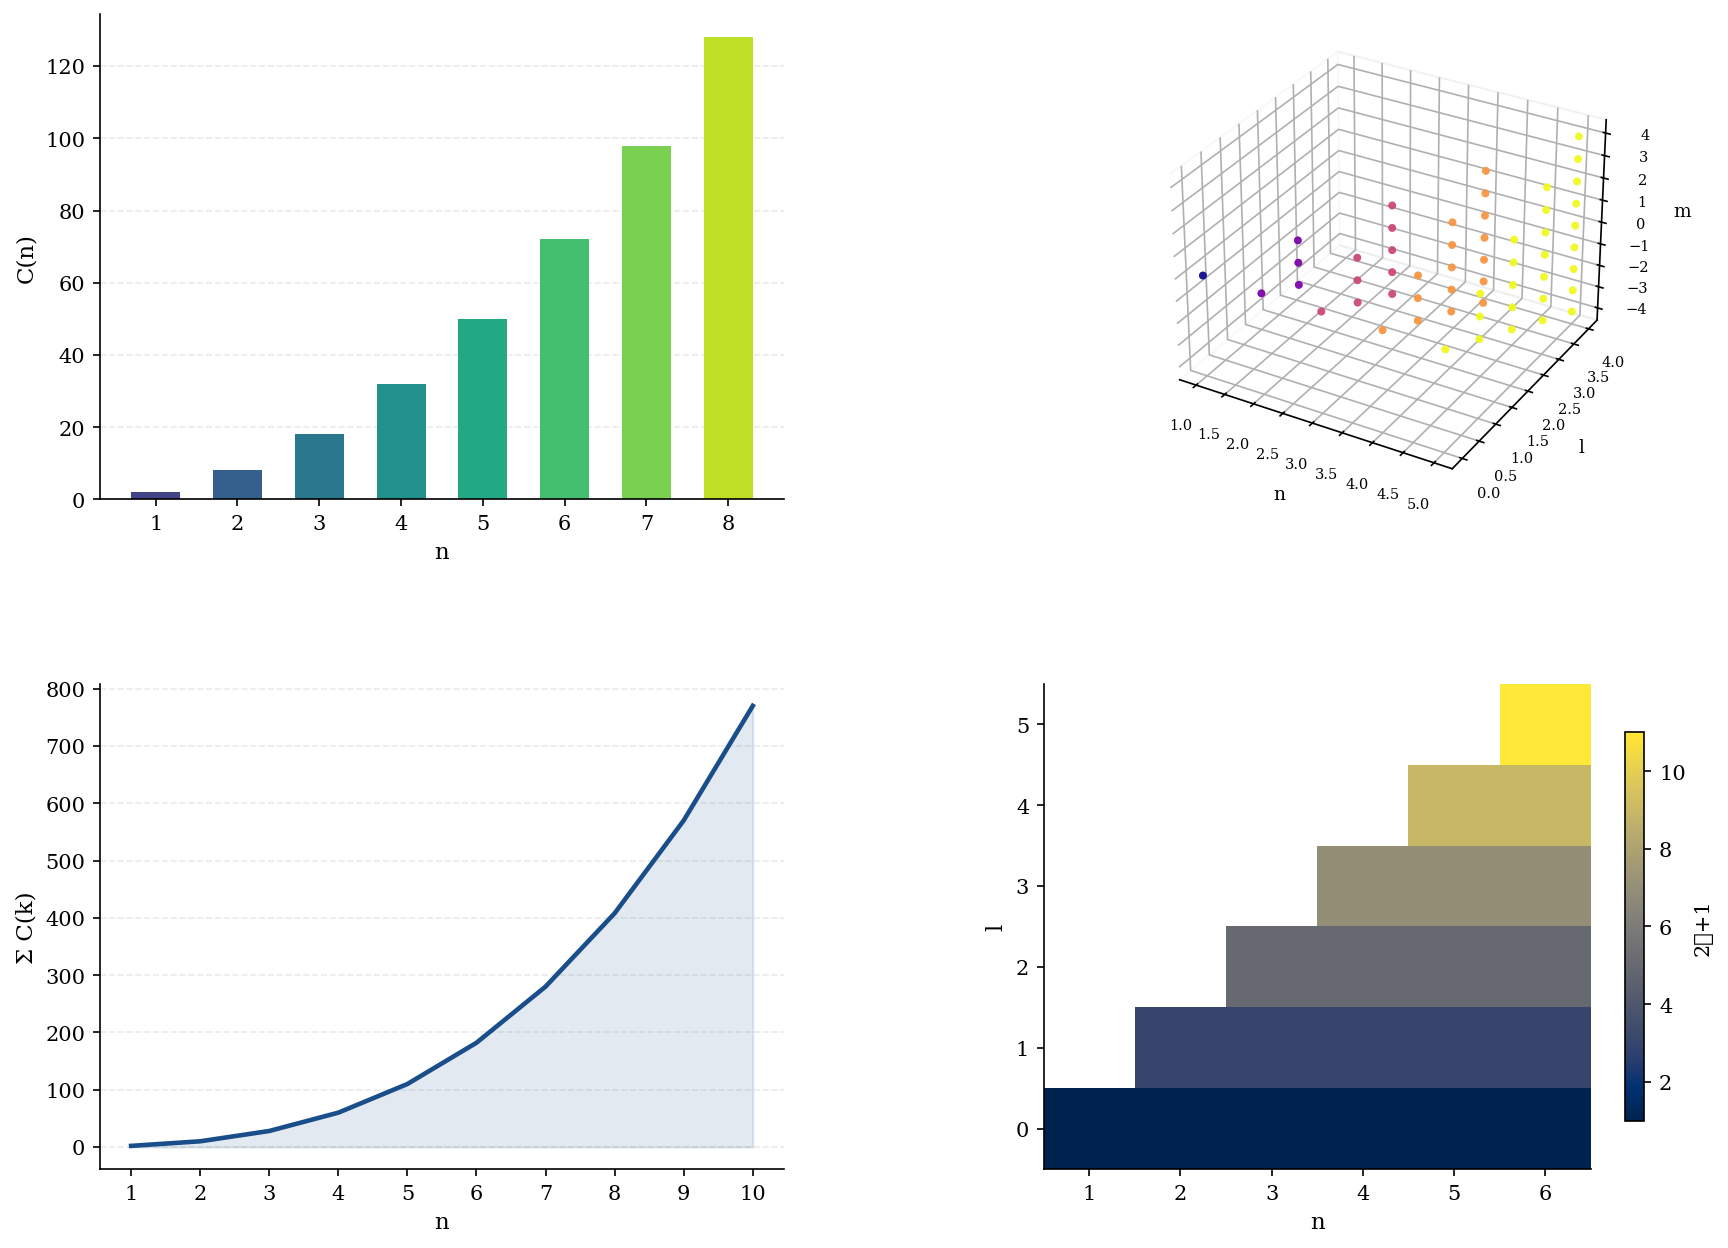
\includegraphics[width=\textwidth]{panel1_partition_geometry.png}
    \caption{\textbf{Partition Space Geometry.}
    (\textbf{A})~Shell capacity $C(n) = 2n^2$ for partition depths
    $n = 1, \ldots, 8$.  Each bar counts the number of valid coordinate
    quadruples $(\ell, m, s)$ at depth $n$: $\ell$ ranges over
    $\{0, \ldots, n-1\}$, $m$ over $\{-\ell, \ldots, +\ell\}$, and
    $s \in \{-\tfrac{1}{2}, +\tfrac{1}{2}\}$, giving
    $2\sum_{\ell=0}^{n-1}(2\ell+1) = 2n^2$ distinct addresses per shell.
    Bars are coloured from cool (shallow) to warm (deep) to indicate
    structural richness increasing with depth.
    (\textbf{B})~Three-dimensional scatter of all valid partition
    coordinates $(n, \ell, m)$ for $n \leq 5$, with spin parity $s$
    doubling each point's multiplicity.  Each point represents a unique
    node identity in the \srn\ network.  Depth $n$ determines the
    colour; the triangular cross-section at each depth reflects the
    constraint $|\,m\,| \leq \ell < n$.  The geometry is the discrete
    analogue of the hydrogen-atom orbital manifold arising from
    $\mathrm{SO}(3)$ representation theory.
    (\textbf{C})~Cumulative coordinate count
    $\sum_{k=1}^{n} 2k^2 = \tfrac{n(n+1)(2n+1)}{3}$ as a function of
    depth $n$.  By $n = 4$, the address space has $110$ distinct nodes;
    by $n = 6$, it reaches $182$.  The filled area emphasises the
    super-linear growth of the address space with depth.
    (\textbf{D})~Heatmap of the number of valid orientation indices
    $2\ell + 1$ over the $(n, \ell)$ grid for $n, \ell \in \{1,\ldots,6\}$.
    Grey (NaN) cells are structurally forbidden ($\ell \geq n$): they
    cannot be individuated at the given depth.  Permitted cells grow
    darker as $\ell$ increases, reflecting the widening orientation fan.
    The triangular forbidden region is the discrete shadow of the angular
    momentum constraint $\ell \in \{0, \ldots, n-1\}$.}
    \label{fig:panel1}
\end{figure*}

% ── Panel 2: Entropic Floor and Catalytic Dynamics ───────────────────────────

\begin{figure*}[!htbp]
    \centering
    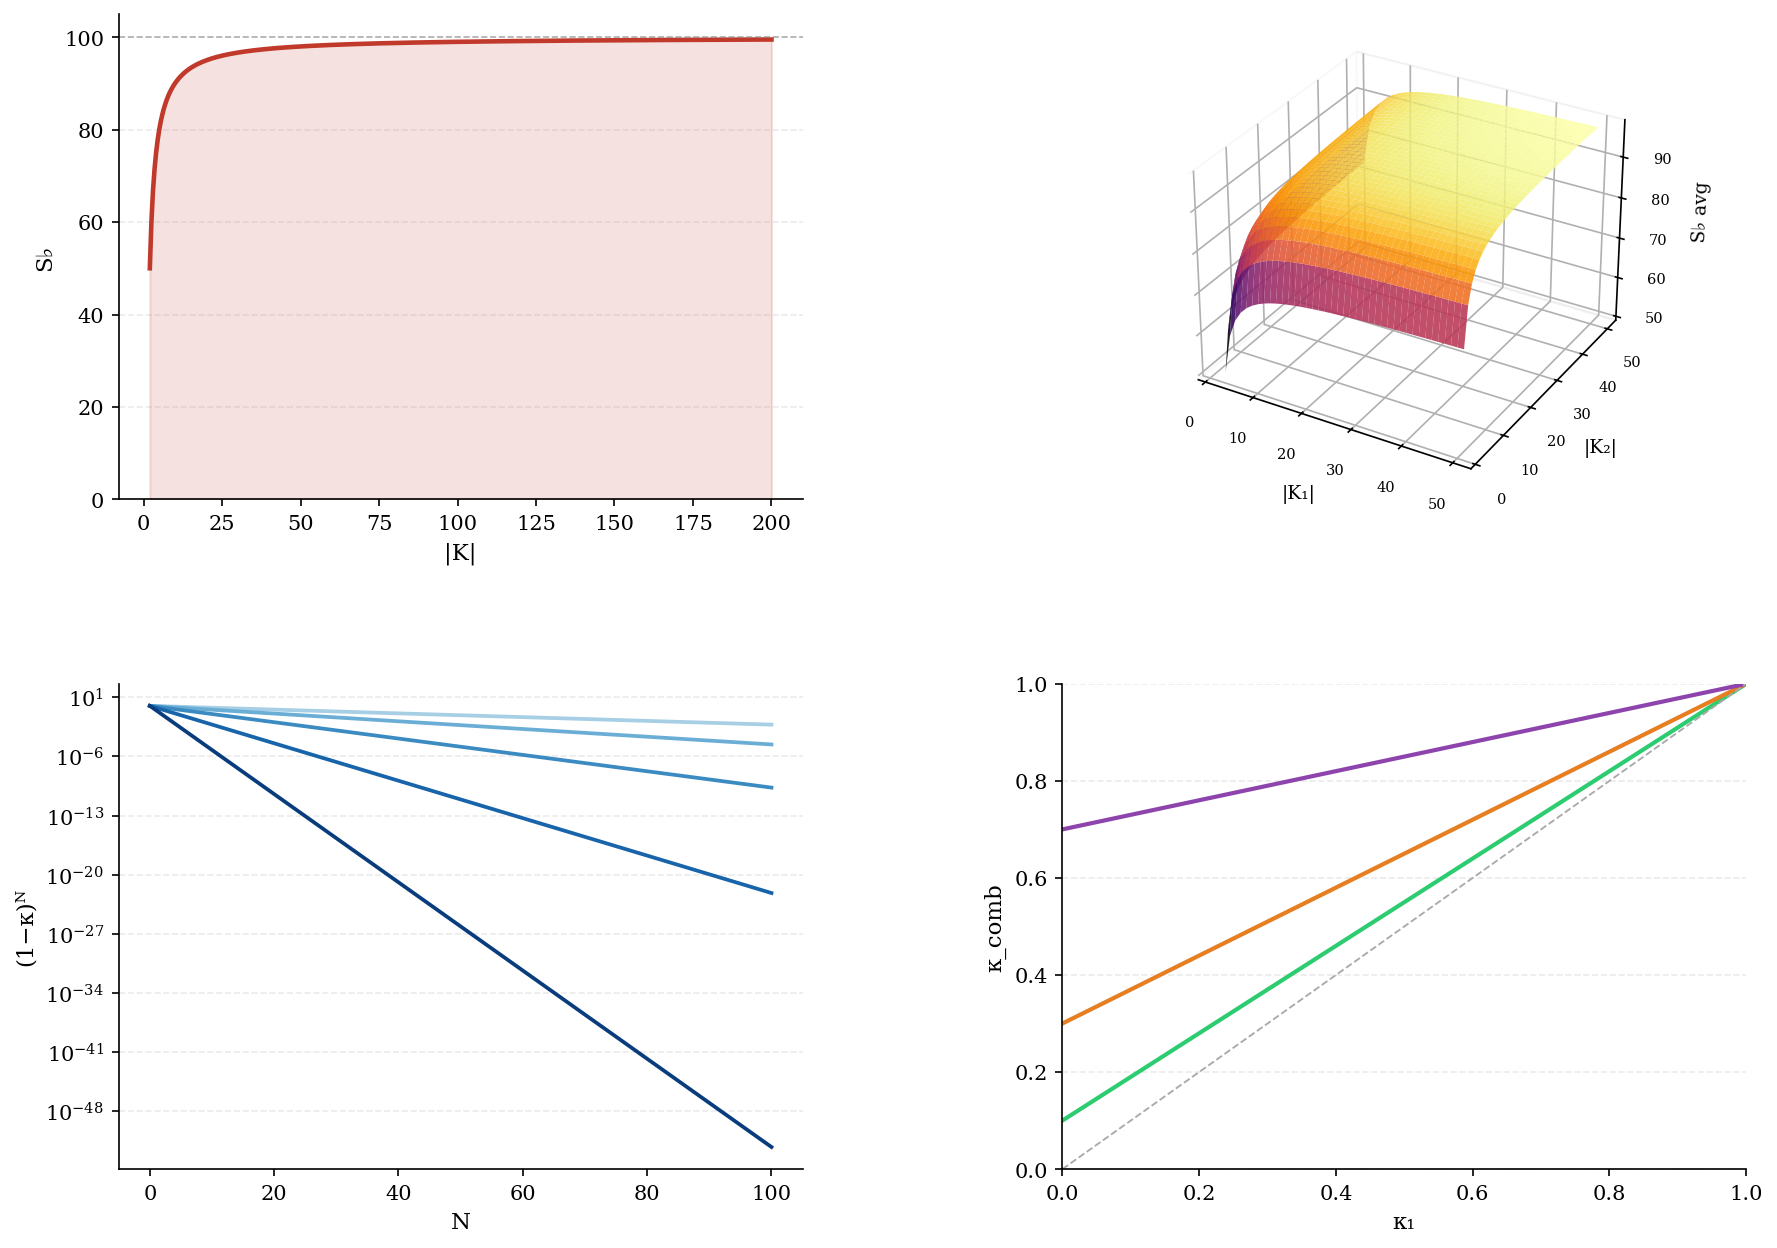
\includegraphics[width=\textwidth]{panel2_entropic_floor.png}
    \caption{\textbf{Entropic Floor and Catalytic Dynamics.}
    (\textbf{A})~The entropic floor $\floor(K) = 100(1 - 1/|K|)$ as a
    function of the receiver's knowledge framework size $|K|$, for
    $|K| \in [2, 200]$.  The filled region marks the range of
    achievable S-values.  The dashed line at $\floor = 100$ is the
    unattainable limit: perfect knowledge requires $|K| = \infty$.  At
    $|K| = 2$, the floor is $50$; at $|K| = 10$, it is $90$; at
    $|K| = 100$, it is $99$.  No finite receiver can close the gap to
    zero error, regardless of expression quality.
    (\textbf{B})~Three-dimensional surface of the average floor
    $\tfrac{1}{2}({\floor}(K_1) + {\floor}(K_2)) =
    50(2 - 1/|K_1| - 1/|K_2|)$ over two independent receiver sizes
    $|K_1|, |K_2| \in [2, 50]$.  The surface rises monotonically in both
    directions and remains strictly below $100$ everywhere.  The two
    receivers each contribute an independent positive floor; the average
    is the relevant quantity for cross-node evaluation, where neither
    receiver can achieve zero error in isolation.
    (\textbf{C})~Log-scale catalytic residual $(1-\kappa)^N$ as a
    function of step count $N \in [0, 100]$ for five catalyst strengths
    $\kappa \in \{0.05, 0.1, 0.2, 0.4, 0.7\}$ (light to dark).  All
    curves converge to zero, confirming the Borel-Cantelli analogue
    (Theorem~\ref{thm:catalyst}): repeated application of any catalyst
    with $\kappa > 0$ drives the residual to zero exponentially fast.
    The rate is $(1-\kappa)$ per step: a catalyst of strength $0.7$
    reduces the residual to $< 10^{-5}$ within $30$ steps; one of
    strength $0.05$ requires $\sim 200$ steps for the same reduction.
    (\textbf{D})~Composite catalytic power
    $\kappa_{\mathrm{comb}}(\kappa_1, \kappa_2)
    = 1 - (1 - \kappa_1)(1 - \kappa_2)$ as $\kappa_1$ varies over
    $[0,1]$ for three fixed values $\kappa_2 \in \{0.1, 0.3, 0.7\}$
    (green, orange, purple).  The diagonal reference line marks
    $\kappa_{\mathrm{comb}} = \kappa_1$.  Every curve lies strictly
    above the diagonal for $\kappa_1 \in (0,1)$, confirming that
    combining two catalysts always outperforms either alone.  A locally
    infeasible catalyst ($\kappa_2$ from a node where $S = 100$) retains
    positive composite power by the Miracle Principle
    (Corollary~\ref{cor:miracle}).}
    \label{fig:panel2}
\end{figure*}

% ── Panel 3: Composition Inflation ───────────────────────────────────────────

\begin{figure*}[!htbp]
    \centering
    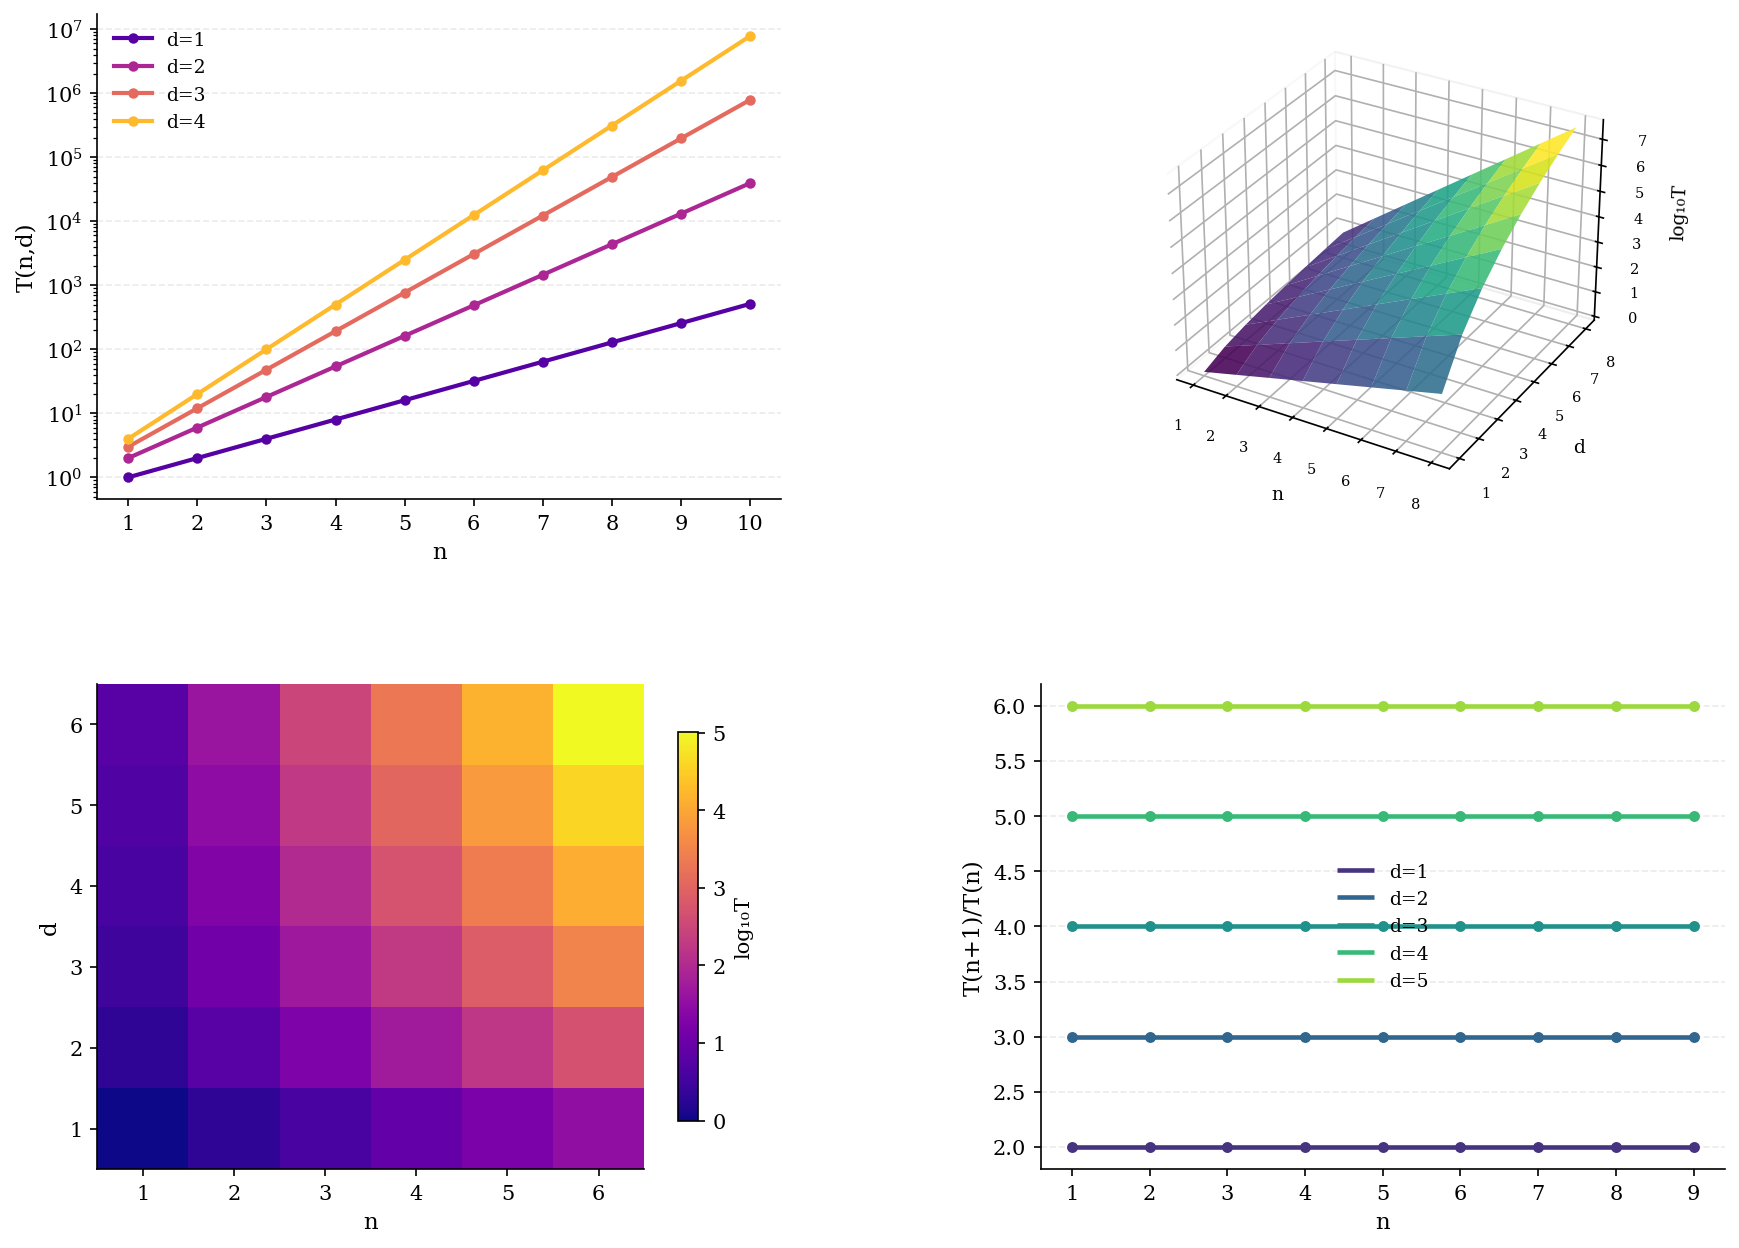
\includegraphics[width=\textwidth]{panel3_composition_inflation.png}
    \caption{\textbf{Composition Inflation $T(n,d) = d(1+d)^{n-1}$.}
    (\textbf{A})~Log-scale growth of $T(n,d)$ versus composition depth
    $n \in \{1, \ldots, 10\}$ for operator counts $d \in \{1, 2, 3, 4\}$.
    All curves are strictly exponential in $n$; the base $(1+d)$
    increases with $d$, so higher operator counts produce faster
    trajectory proliferation.  At $n = 10$ and $d = 4$, the number of
    distinguishable labeled trajectories exceeds $2 \times 10^6$.  The
    linear regime ($n = 1$, where $T = d$ regardless of base) is the
    unique fixed point visible at the left edge.
    (\textbf{B})~Three-dimensional surface of $\log_{10} T(n,d)$ over
    $(n, d) \in \{1, \ldots, 8\}^2$.  The surface is coloured by height:
    cool shades indicate few trajectories; warm shades indicate many.
    The exponential dependence on $n$ and the linear-then-exponential
    dependence on $d$ produce a surface that rises steeply in both
    directions, but more steeply along $n$ for fixed $d > 1$.
    (\textbf{C})~Heatmap of $\log_{10} T(n,d)$ for
    $(n, d) \in \{1,\ldots,6\}^2$.  Each cell is coloured by the
    base-10 logarithm of the trajectory count.  The heatmap reveals
    the multiplicative structure: moving one step right (increasing $n$
    by $1$) multiplies $T$ by $(1+d)$; moving one step up (increasing
    $d$ by $1$) adds an additional factor that varies with $n$.  The
    fastest-growing cell at $(n=6, d=6)$ has $T = 6 \cdot 7^5 \approx
    7 \times 10^4$ trajectories.
    (\textbf{D})~Growth ratio $T(n+1, d) / T(n, d) = 1 + d$ as a
    function of $n$ for $d \in \{1, 2, 3, 4, 5\}$.  Each curve is a
    horizontal line, confirming that the ratio is exactly constant in
    $n$: the exponential base $(1+d)$ is independent of depth.  This
    is a structural consequence of the binomial identity underlying the
    Composition Inflation theorem (Theorem~\ref{thm:inflation}), not
    a numerical accident.  Dots mark the integer values of $n$ where
    the ratio was evaluated.}
    \label{fig:panel3}
\end{figure*}

% ── Panel 4: Forest Dynamics and Receiver-Relative Evaluation ────────────────

\begin{figure*}[!htbp]
    \centering
    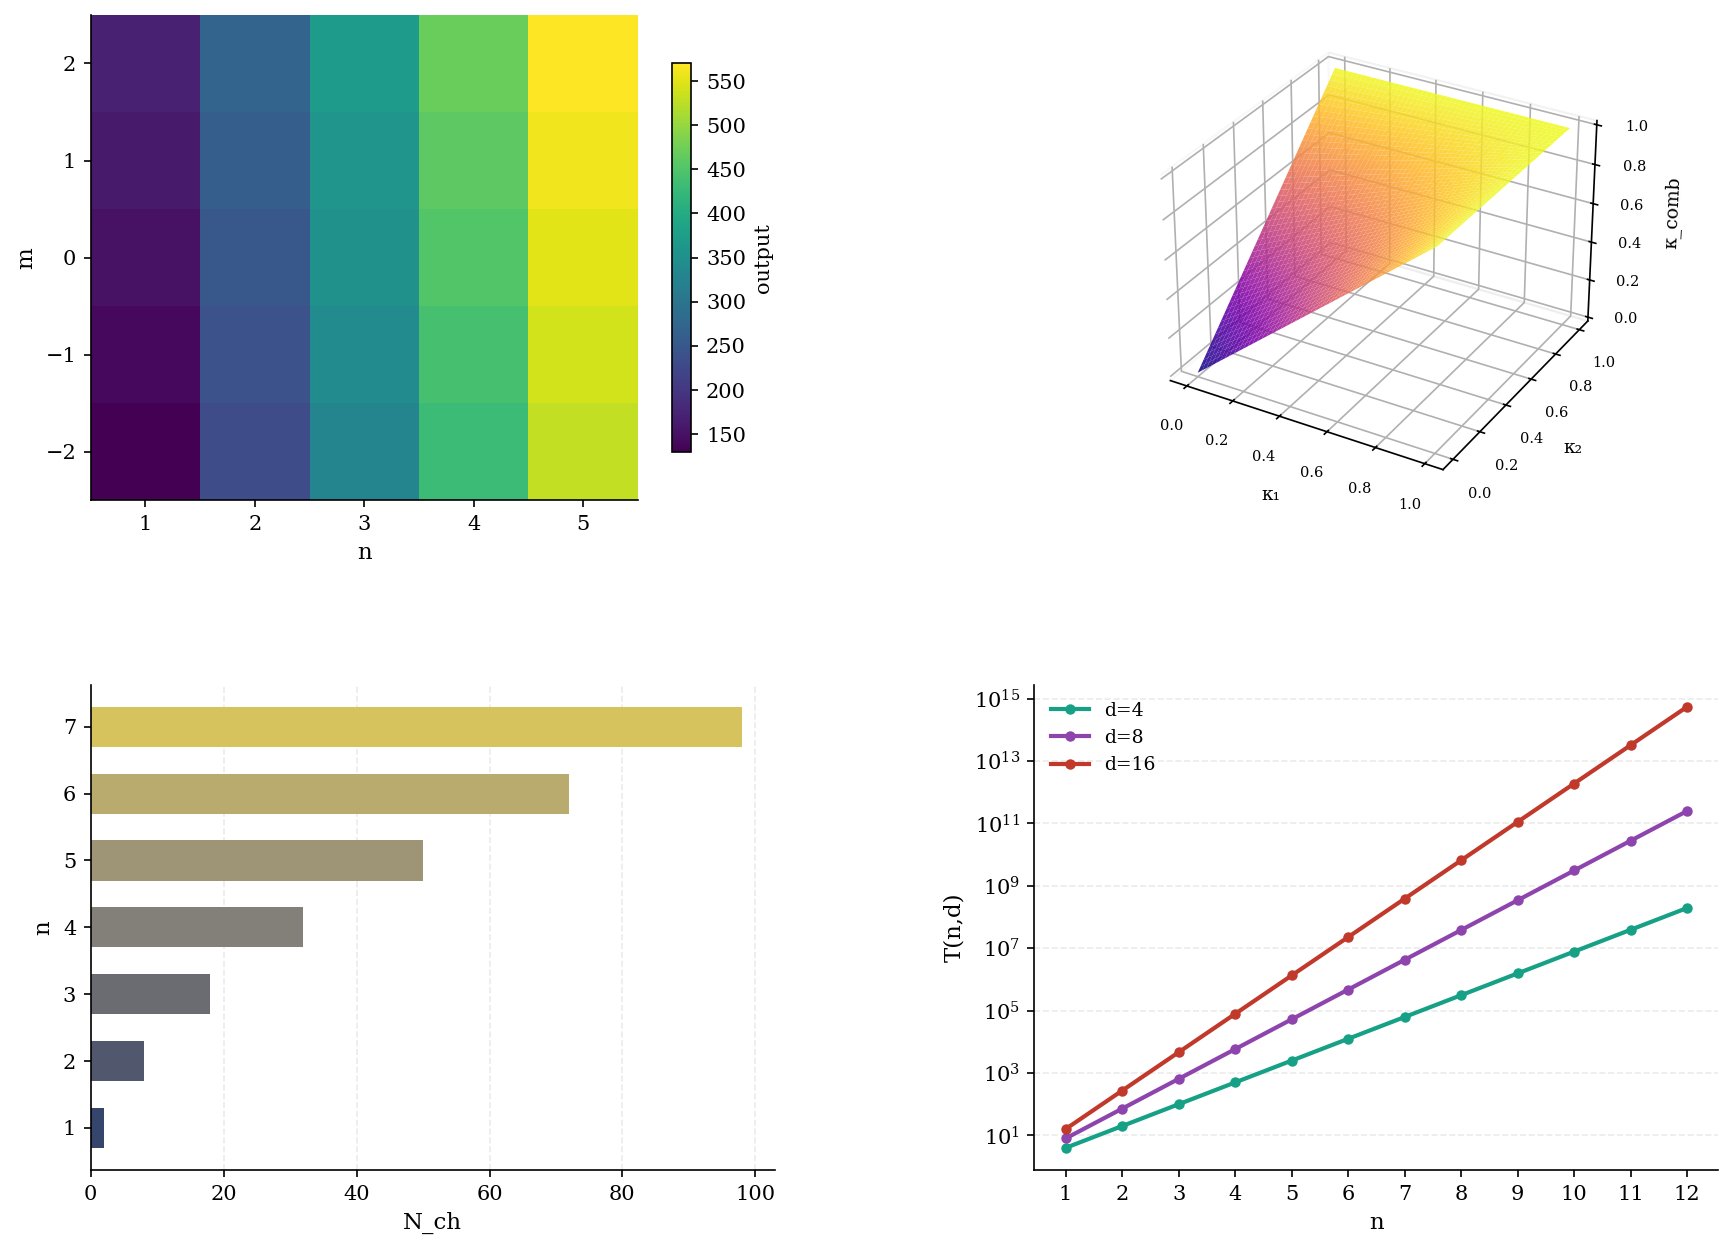
\includegraphics[width=\textwidth]{panel4_forest_dynamics.png}
    \caption{\textbf{Forest Dynamics and Receiver-Relative Evaluation.}
    (\textbf{A})~Heatmap of the receiver-relative output
    $v = 100n + 10m + M$ (with partition count $M = 50$ fixed)
    across the $(n, m)$ node grid, $n \in \{1,\ldots,5\}$,
    $m \in \{-2,-1,0,+1,+2\}$.  Every cell yields a distinct value:
    no two nodes evaluate the same expression to the same result.
    This is a direct numerical illustration of
    Theorem~\ref{thm:rr} (Receiver-Relativity): the same \srn\
    expression produces different output at every node in the network,
    with all outputs simultaneously valid.  The colour gradient
    encodes the output value; no central authority reconciles the
    divergent results.
    (\textbf{B})~Three-dimensional surface of composite catalytic power
    $\kappa_{\mathrm{comb}}(\kappa_1, \kappa_2)
    = 1 - (1 - \kappa_1)(1 - \kappa_2)$ over $(\kappa_1, \kappa_2)
    \in [0,1]^2$.  The surface is bounded in $[0,1]^2$, rises
    monotonically in both arguments, and reaches $1$ only at the corner
    $(\kappa_1, \kappa_2) = (1, 1)$.  The curvature of the surface
    reflects the multiplicative—not additive—structure of catalytic
    combination: a second catalyst of strength $\kappa_2$ acts on the
    \emph{residual} $1 - \kappa_1$, not on the full domain.
    (\textbf{C})~Forced channel count $N_{\mathrm{ch}} = 2n^2$ per
    partition depth $n \in \{1,\ldots,7\}$, shown as horizontal bars.
    These are the independent communication channels structurally
    mandated by the node's topology (Theorem~\ref{thm:channels}): a
    node at depth $4$ must support $32$ independent channels; at depth
    $7$, it must support $98$.  The channel count is not a design
    parameter; it is forced by the cycle rank of the contact graph on
    the shell elements.  Bars are coloured by depth.
    (\textbf{D})~Trajectory encoding capacity $T(n, d)$ for channel
    counts $d \in \{4, 8, 16\}$ and composition depths $n = 1,\ldots,12$,
    on a log scale.  Each curve represents the number of distinguishable
    \srn\ expressions encodable as timing trajectories at that channel
    count.  At $n = 12$ and $d = 16$, the capacity reaches
    $T = 16 \cdot 17^{11} \approx 3.4 \times 10^{13}$ distinct
    expressions.  The channel count $d = 4$ corresponds to a minimal
    four-channel node (depth $n = 1$, $N_{\mathrm{ch}} = 2$); $d = 16$
    corresponds to a depth-$3$ node ($N_{\mathrm{ch}} = 18$).  Existing
    internet infrastructure, which already measures timing deviations
    $\Delta P(k)$ at nanosecond resolution across multiple channels,
    operates comfortably in this regime.}
    \label{fig:panel4}
\end{figure*}
